%!TEX root = handout.tex

\newpage
\section{Label-free quantification of metabolites}

\subsection{Introduction}
Quantitation and identification of chemical compounds are basic tasks in metabolomic studies. In this tutorial session we construct a UPLC-MS based, label-free quantitation and identification workflow. Following quantitation and identification we then perform statistical downstream analysis to detect quantitation values that differ significantly between two conditions. This approach can, for example, be used to detect biomarkers. Here, we use two spike-in conditions of a dilution series (0.5 mg/l and 10.0 mg/l, male blood background, measured in triplicates) comprising seven isotopically labeled compounds. The goal of this tutorial is to detect and quantify these differential spike-in compounds against the complex background.

%\begin{figure}[htbp]
%  \centering
%  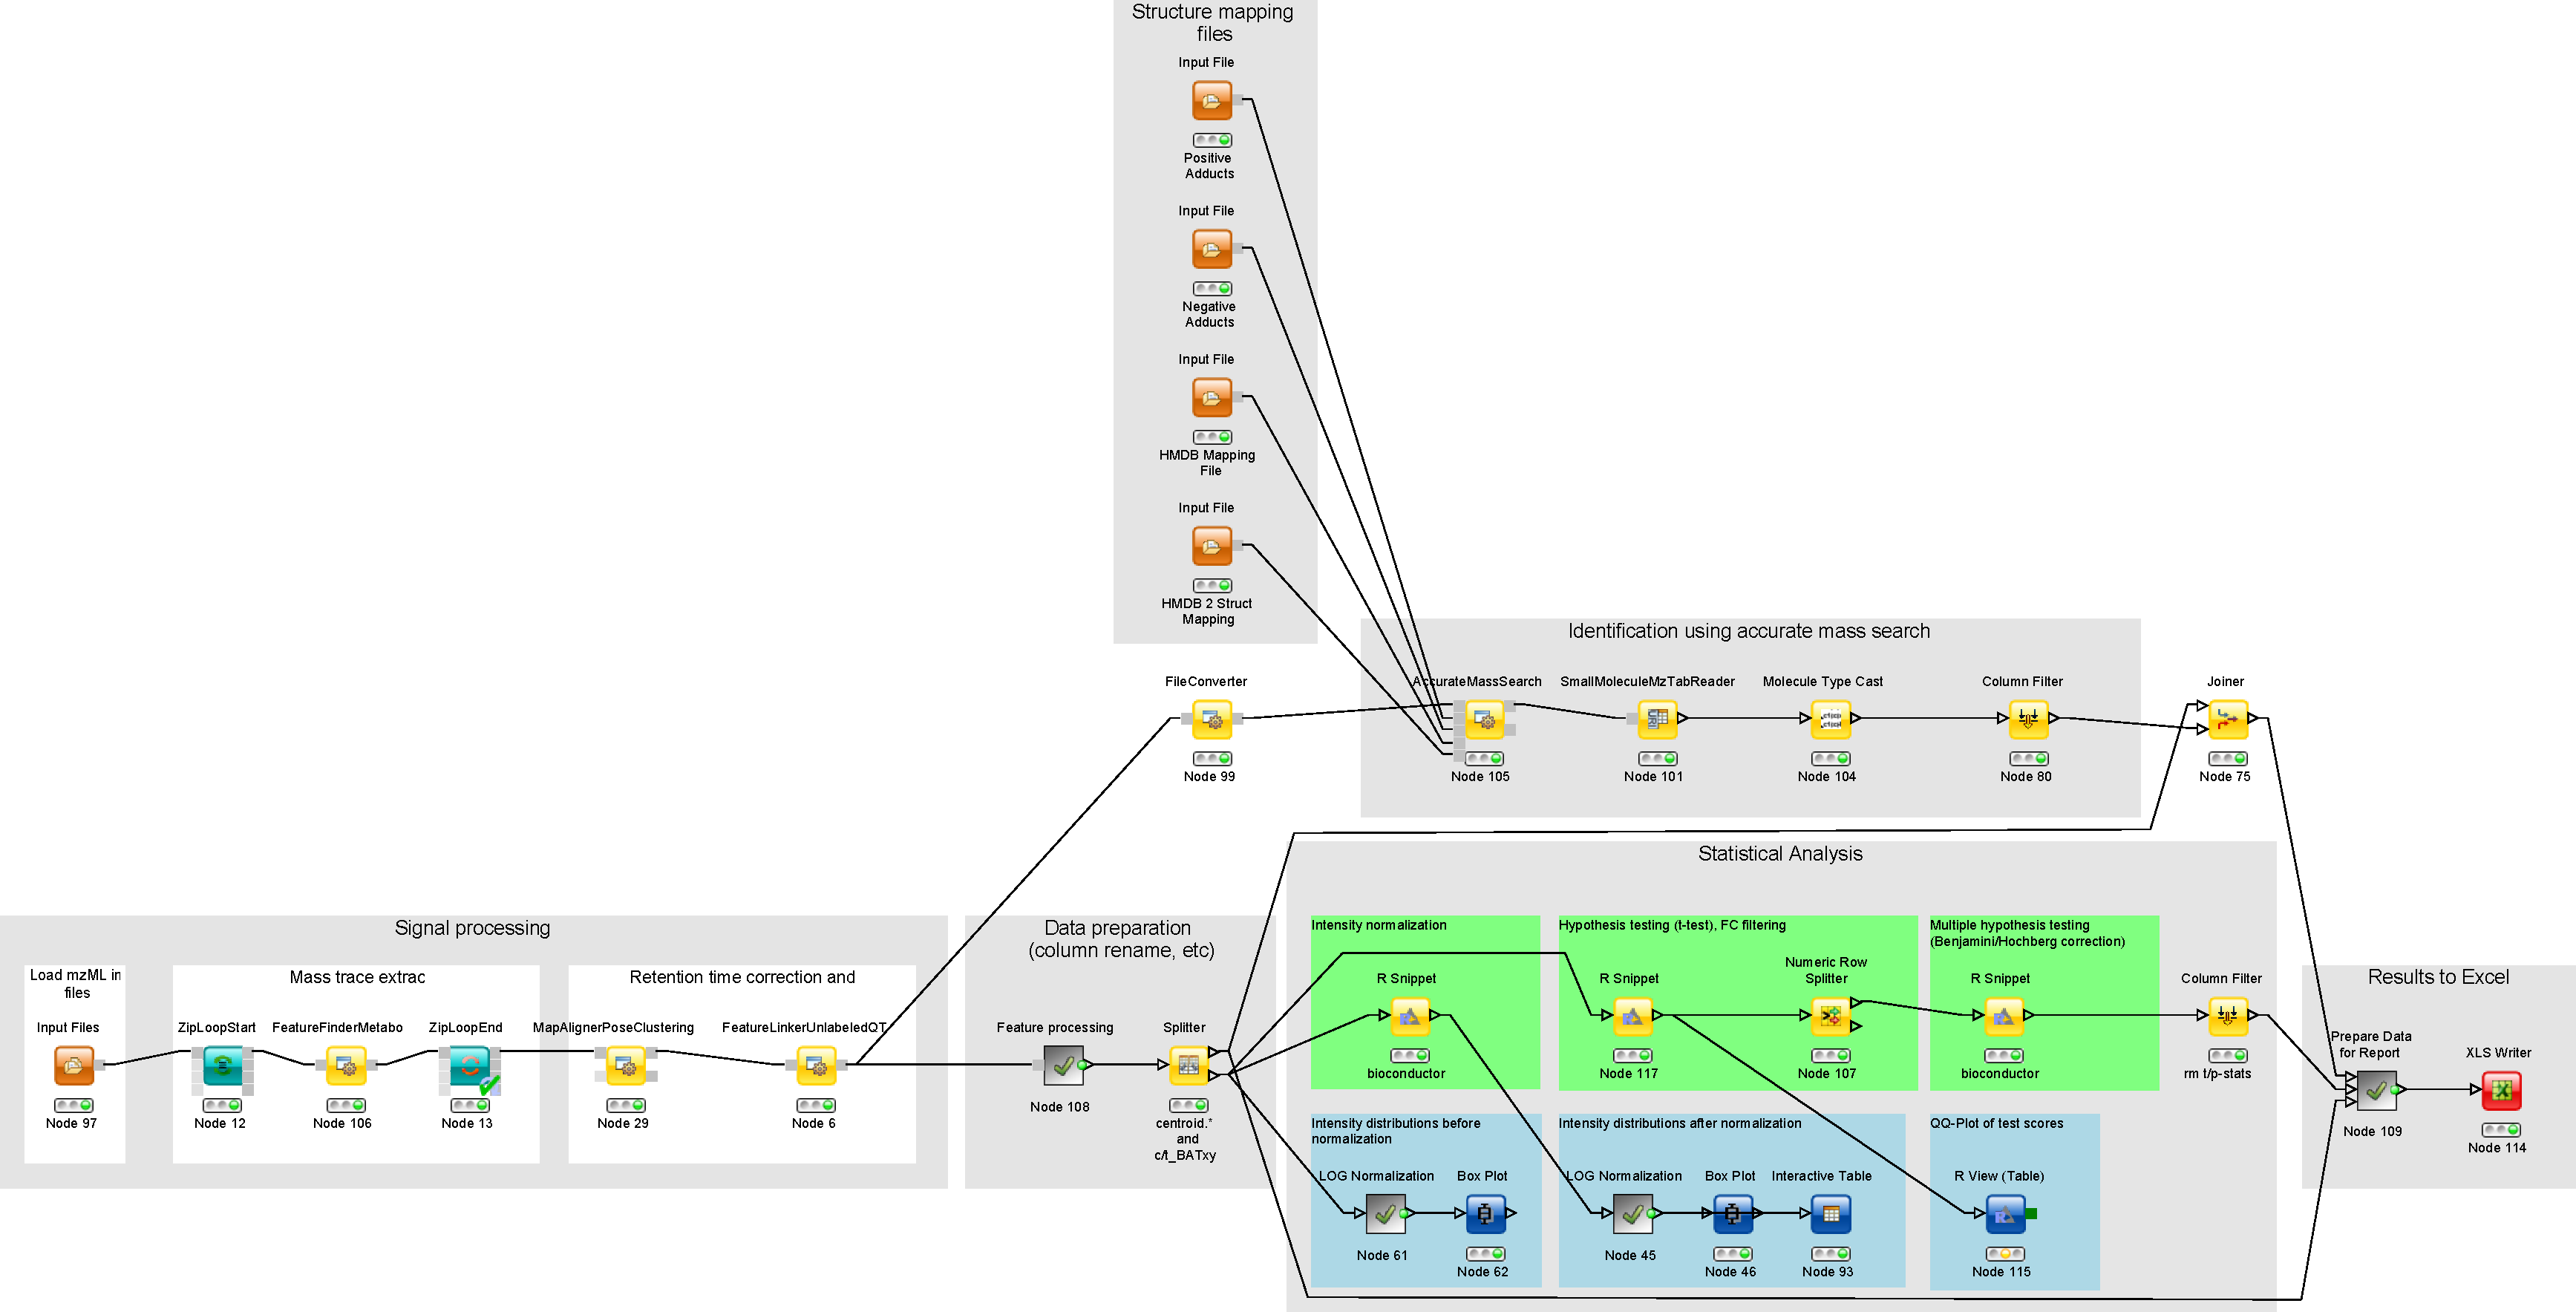
\includegraphics[width=0.85\textwidth]{graphics/metabo/metabo_workflow}
%  \caption{Complete label-free metabolomics quantification workflow}
%  \label{fig:consensusid}
%\end{figure}

\subsection{Basics of non-targeted metabolomics data analysis}

For the metabolite quantification we choose an approach similar to the one used for peptides, but this time based on the OpenMS \KNIMENODE{FeatureFinderMetabo} method. This feature finder again collects peak picked data into individual mass traces. The reason why we need a different feature finder for metabolites lies in the step after trace detection: the aggregation of isotopic traces belonging to the same compound ion into the same feature. Compared to peptides with their averagine model, small molecules have very different isotopic distributions. To group small molecule mass traces correctly, an aggregation model tailored to small molecules is thus needed. 

\begin{itemize}
\item
Create a new workflow called for instance "Metabolomics".
\item
Add an \KNIMENODE{Input File} node and configure it with one mzML file from the \directory{Example\_Data / Metabolomics / datasets}.
\item
Add a \KNIMENODE{FeatureFinderMetabo} node (from \menu{Community Nodes > OpenMS > Quantitation} and connect the first output port of the \KNIMENODE{Input File} to the \KNIMENODE{FeatureFinderMetabo}.
\item
For an optimal result adjust the following settings.
Please note that some of these are advanced parameters.
\item
Connect a \KNIMENODE{Output Folder} to the output of the \KNIMENODE{FeatureFinderMetabo} (see Fig.~\ref{fig:minimal_FFM_wf}).

\begin{figure}[!htbp]
  \centering
  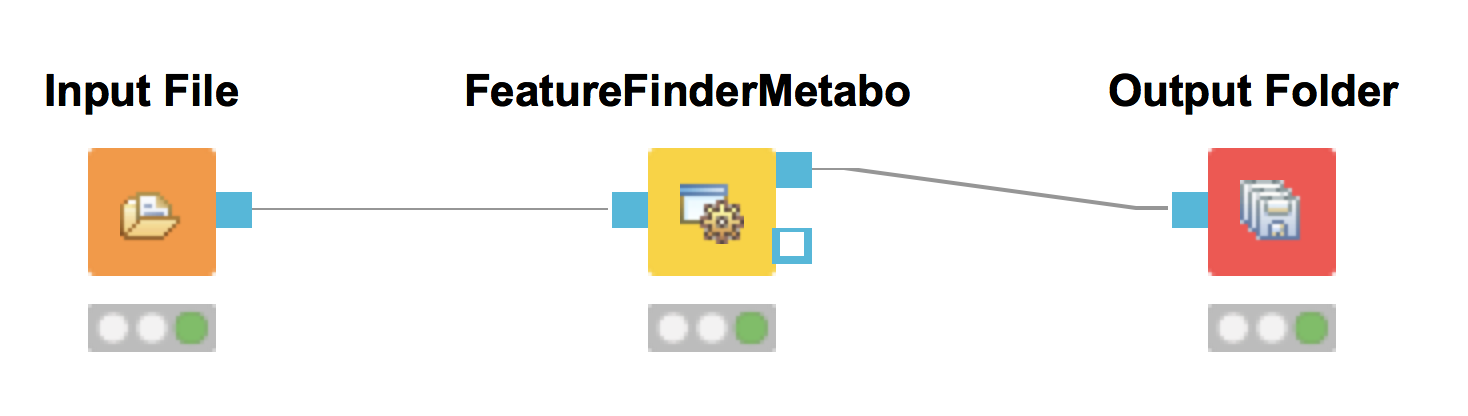
\includegraphics[width=0.5\textwidth]{graphics/metabo/minimal_FFM_wf.png}
  \caption{FeatureFinderMetabo workflow.}
  \label{fig:minimal_FFM_wf}
\end{figure}

In the following advanced parameters will be \hl{highlighted}. These parameter can be altered if the \menu{Show advanced parameter} field in the specific tool is activated (right bottom corner - see ~\ref{KNIME_concepts}). 

\begin{center}
\begin{tabular}{l|l}
\textbf{parameter} & \textbf{value} \\ \hline
\textit{algorithm $\rightarrow$ common $\rightarrow$ chrom\_fwhm} & $8.0$ \\
\textit{algorithm $\rightarrow$ mtd $\rightarrow$ trace\_termination\_criterion} & sample\_rate \\
\hl{\textit{algorithm $\rightarrow$ mtd $\rightarrow$ min\_trace\_length}} & $3.0$ \\
\hl{\textit{algorithm $\rightarrow$ mtd $\rightarrow$ max\_trace\_length}} & $600.0$\\
\textit{algorithm $\rightarrow$ epd $\rightarrow$ width\_filtering} & off \\
\textit{algorithm $\rightarrow$ ffm $\rightarrow$ report\_convex\_hulls} & true
\end{tabular}
\end{center}
\end{itemize}

The parameters change the behavior of \KNIMENODE{FeatureFinderMetabo} as follows:
\begin{itemize}
\item \textbf{chrom\_fwhm}: The expected chromatographic peak width in seconds.
\item \textbf{trace\_termination\_criterion}: In the first stage \KNIMENODE{FeatureFinderMetabo} assembles mass traces with a pre-defined mass accuracy. If this parameter is set to 'outlier', the extension of a mass trace is stopped after a predefined number of consecutive outliers is found. If this parameter is set to 'sample\_rate', the extension of a mass trace is stopped once the ratio of collected peaks versus visited spectra falls below the ratio given by min\_sample\_rate.
\item \textbf{min\_trace\_length}: Minimal length of a mass trace in seconds. Choose a small value, if you want to identify low-intensity compounds.
\item \textbf{max\_trace\_length}: Maximal length of a mass trace in seconds. Set this parameter to -1 to disable the filtering by maximal length.
\item \textbf{width\_filtering}: \KNIMENODE{FeatureFinderMetabo} can remove features with unlikely peak widths from the results. If activated it will use the interval provided by the paramters min\_fwhm and max\_fwhm.
\item \textbf{report\_convex\_hulls}: If set to true, convex hulls including mass traces will be reported for all identified features. This increases the output size considerably.
\end{itemize}

\noindent The output file .featureXML can be visualized with TOPPView on top of the used .mzML file - in a so called 	\textit{layer} - to look at the identified features.
\newline
 
\noindent First start TOPPView and open the example .mzML file (see Fig.~\ref{fig:ToppView_1}). Afterwards open the .featureXML output as new layer (see Fig.~\ref{fig:ToppView_2}). The overlay is depcied in Figure~\ref{fig:ToppView_3}. The zoom of the .mzML - .featureXML overlay shows the individual mass traces and the assembly of those in a feature (see Fig.~\ref{fig:ToppView_4}).

\begin{figure}[htbp]
  \centering
  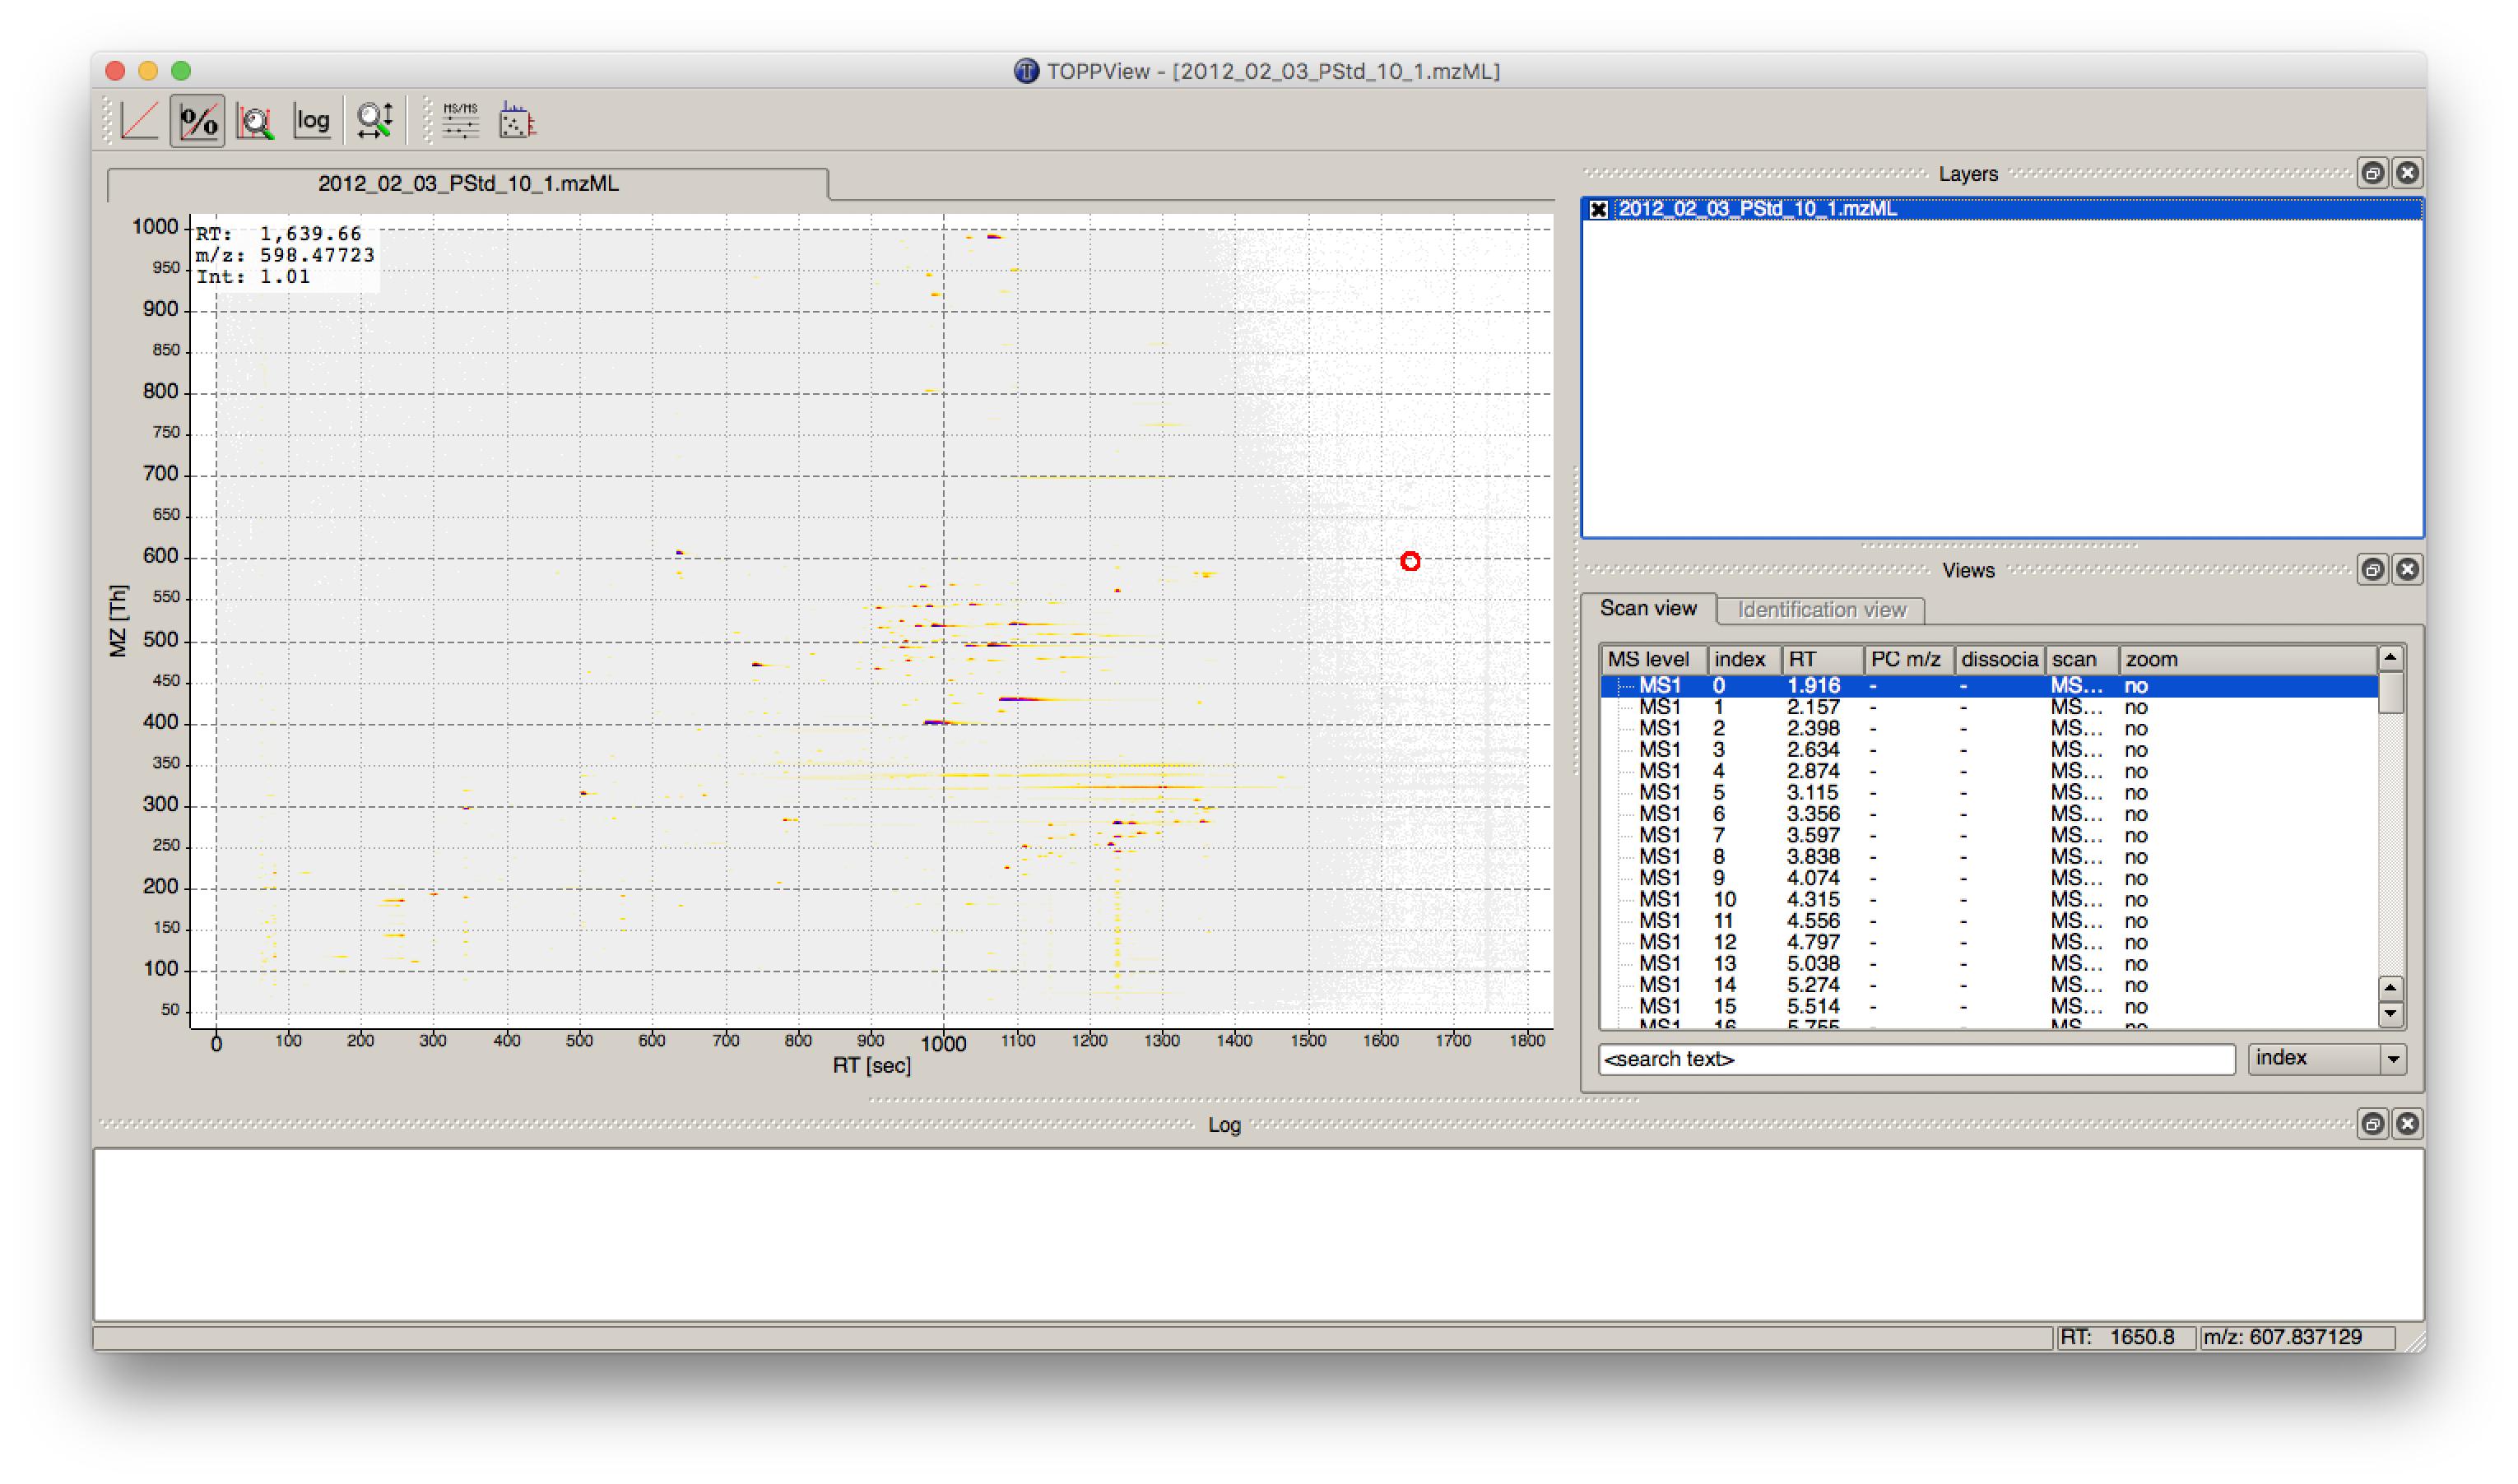
\includegraphics[width=\textwidth]{graphics/metabo/ToppView_1.png}
  \caption{Openend .mzML in TOPPView.}
  \label{fig:ToppView_1}
\end{figure}

\begin{figure}[htbp]
  \centering
  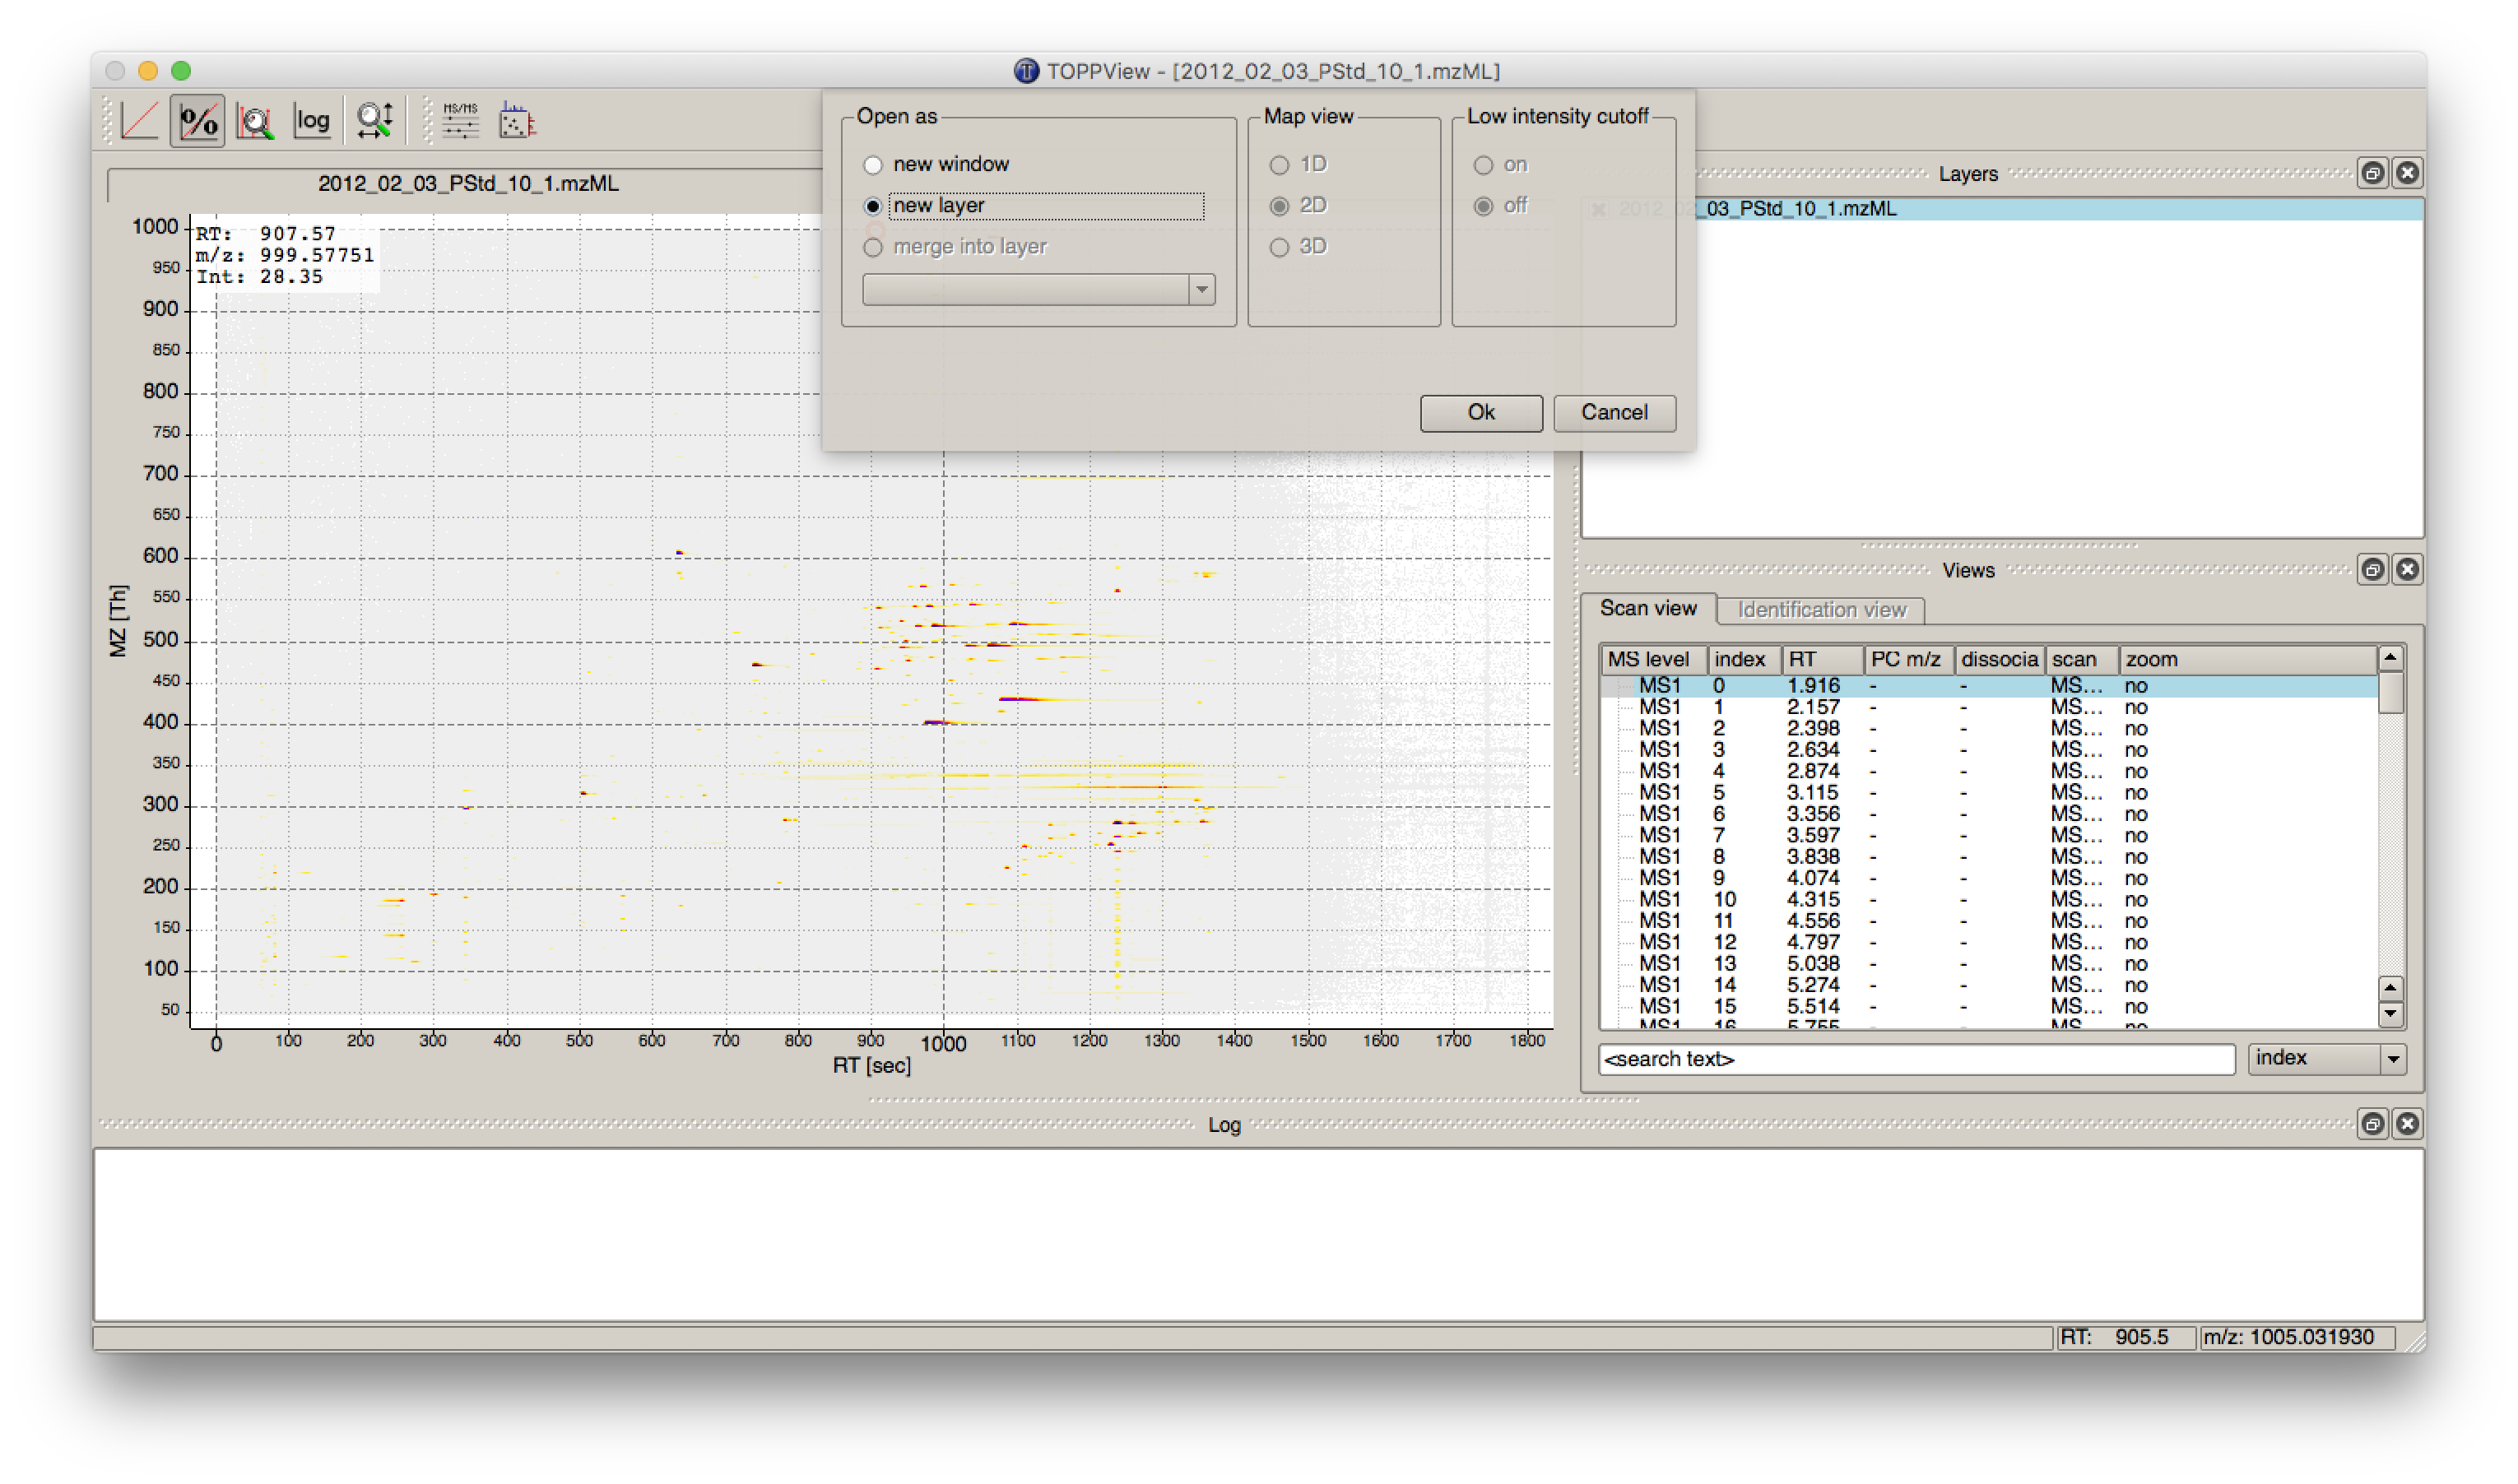
\includegraphics[width=\textwidth]{graphics/metabo/ToppView_2.png}
  \caption{Add new layer in TOPPView.}
  \label{fig:ToppView_2}
\end{figure}

\begin{figure}[htbp]
  \centering
  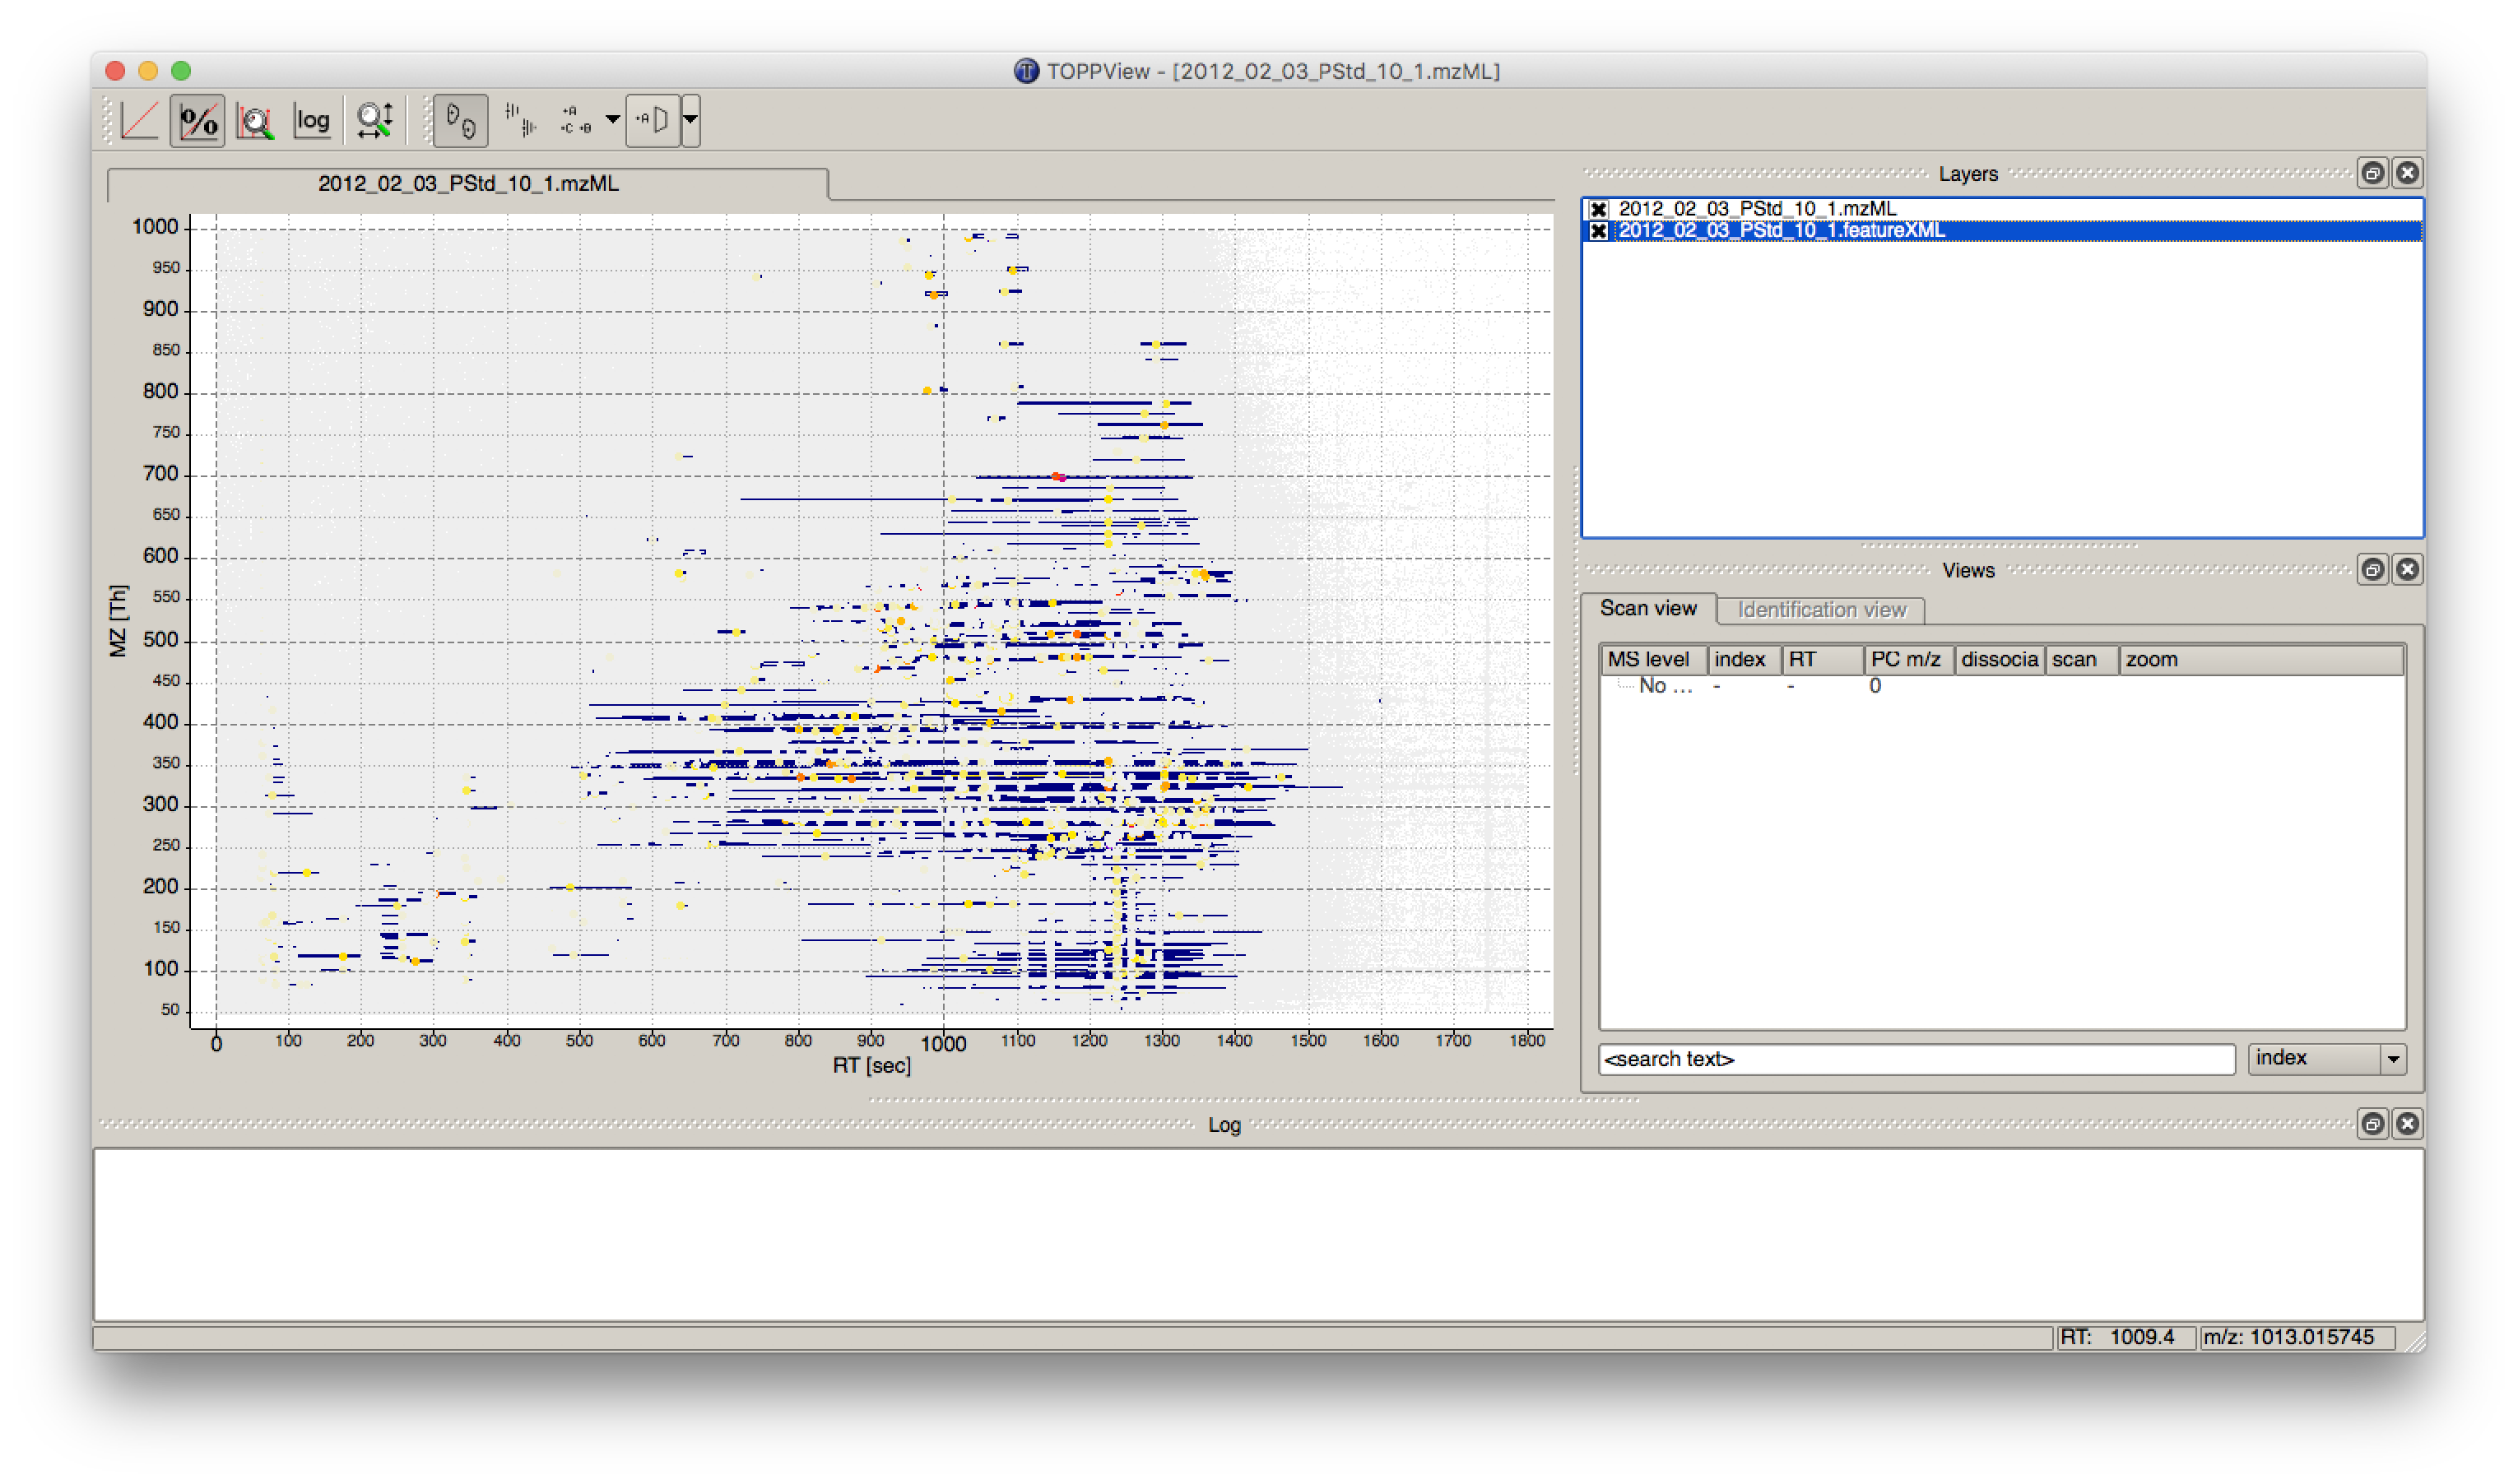
\includegraphics[width=\textwidth]{graphics/metabo/ToppView_3.png}
  \caption{Overlay of the .mzML layer with the .featureXML layer. }
  \label{fig:ToppView_3}
\end{figure}

\begin{figure}[htbp]
  \centering
  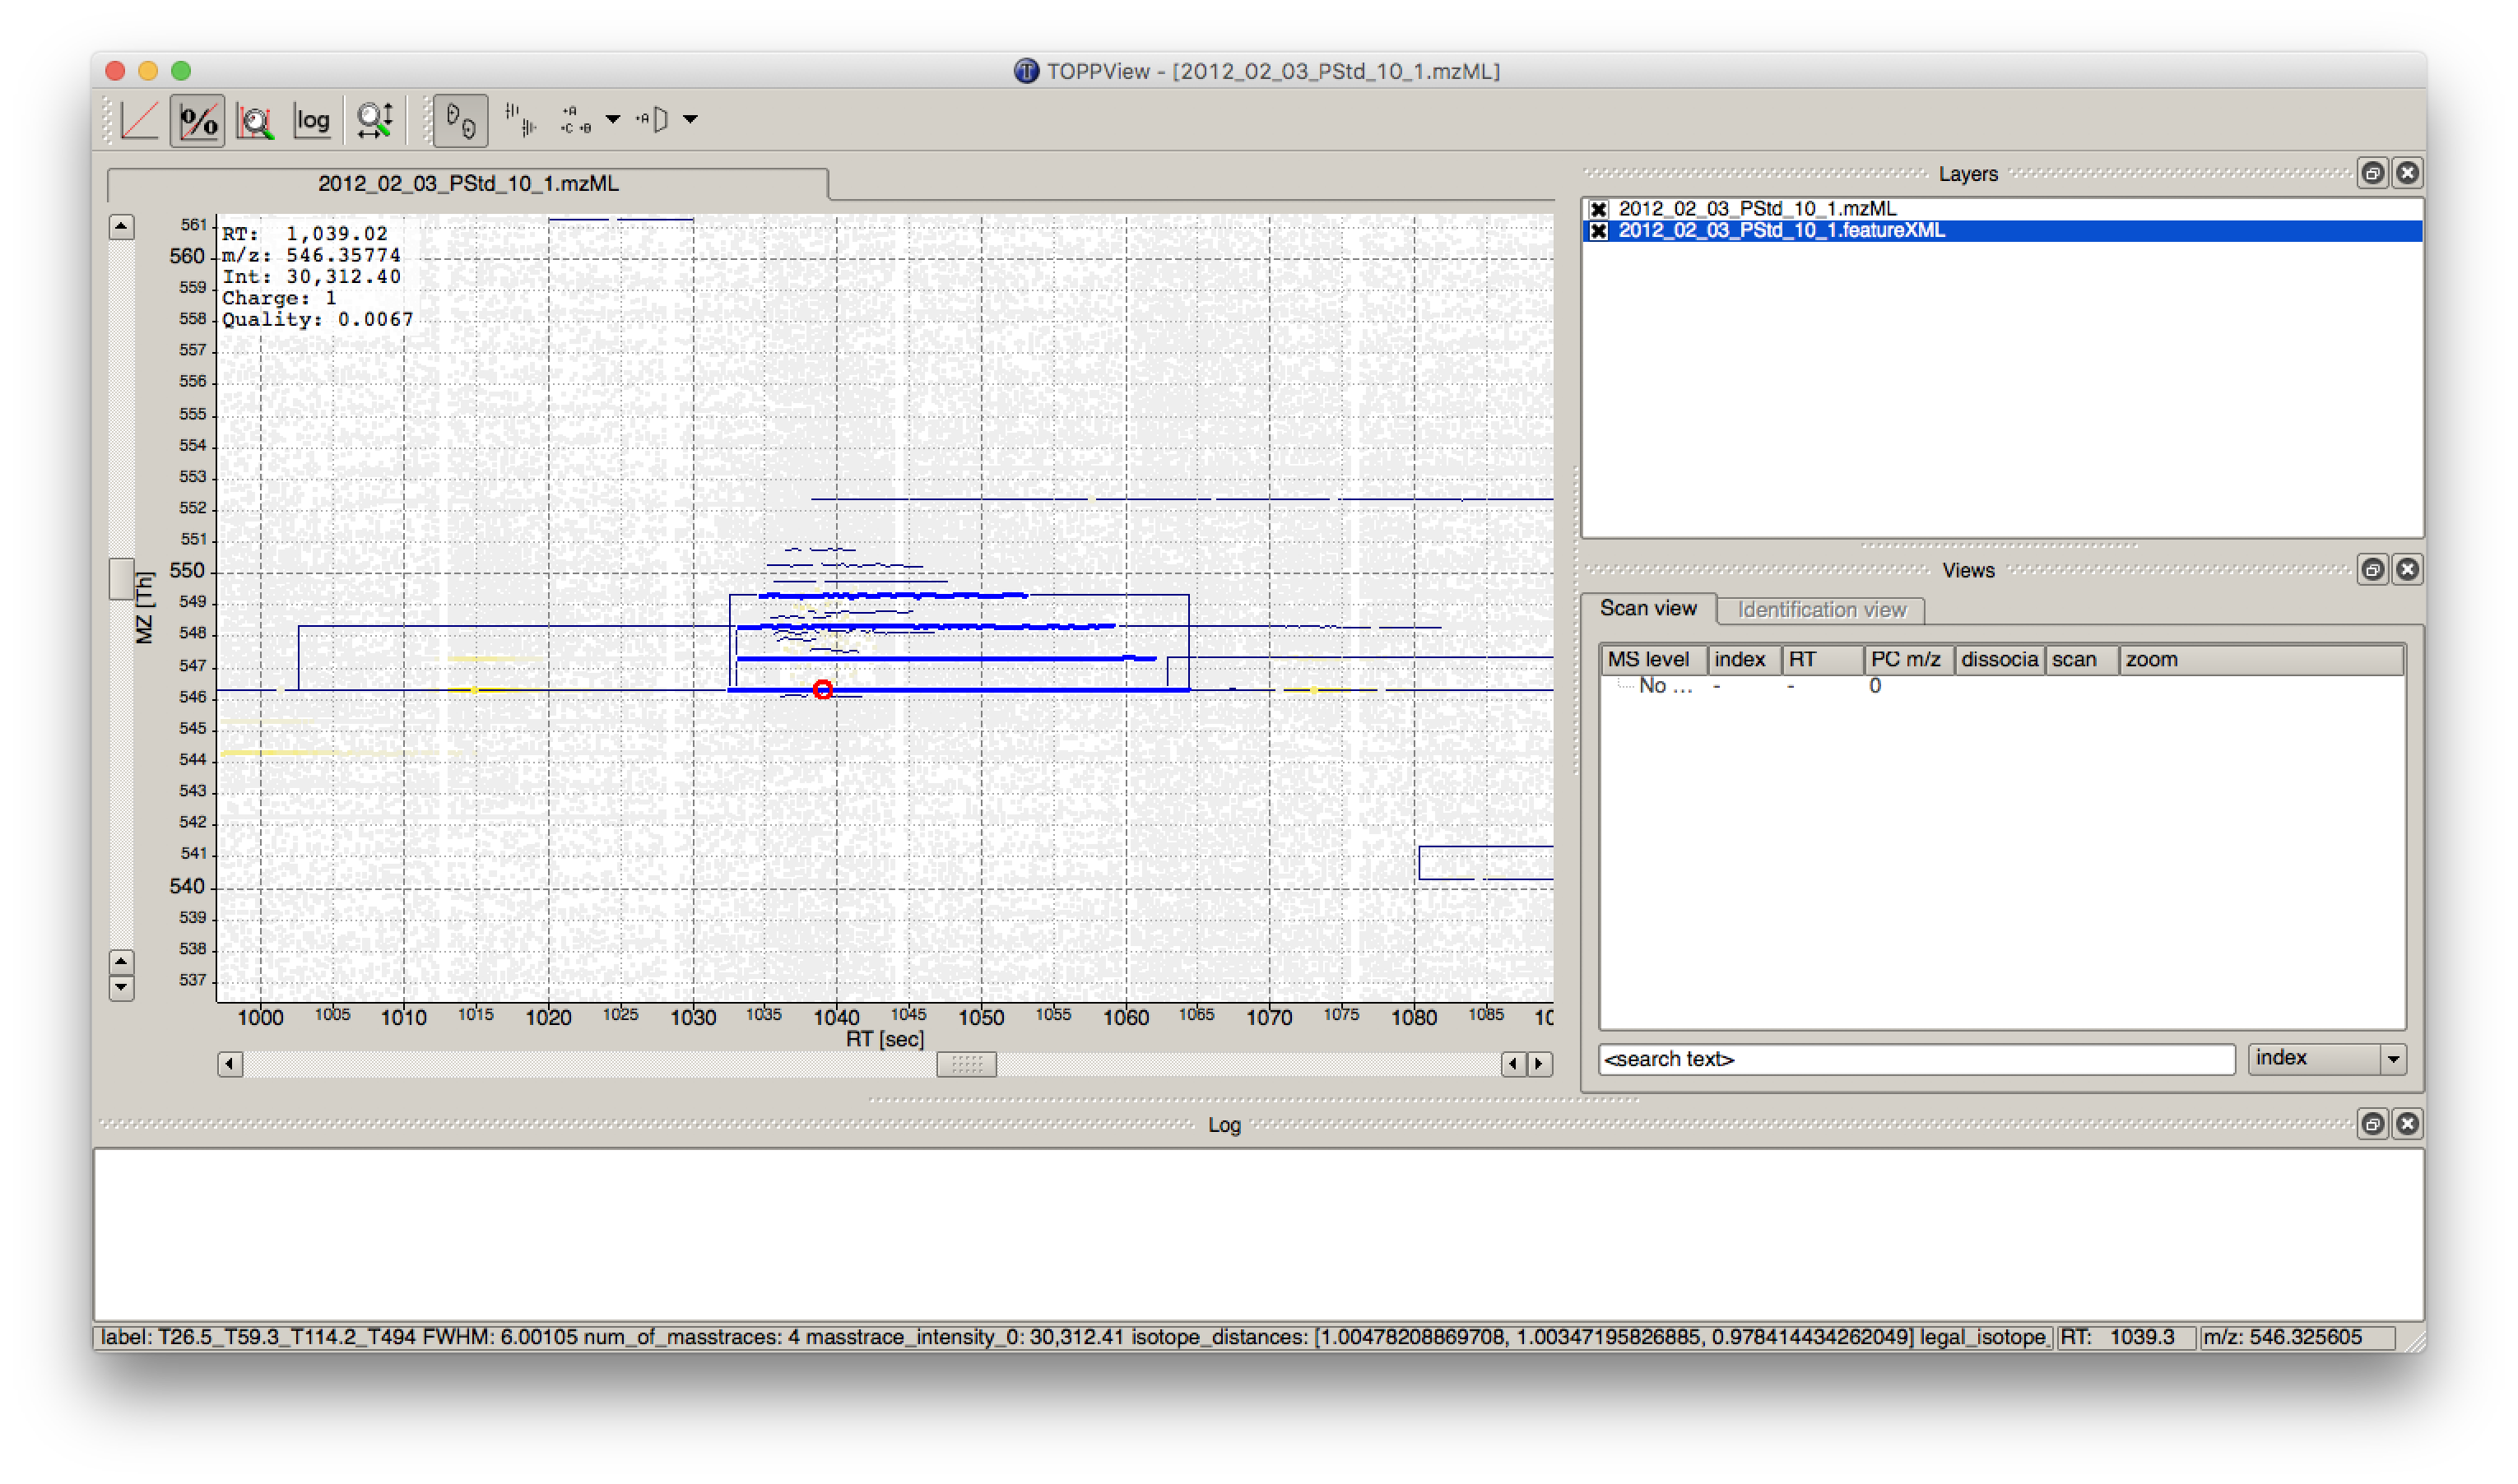
\includegraphics[width=\textwidth]{graphics/metabo/ToppView_4.png}
  \caption{Zoom of the overlay of the .mzML with the .featureXML layer. Here the individual isotope traces (blue lines) are assembled into a feature here shown as convex hull (rectangular box).}
  \label{fig:ToppView_4}
\end{figure}

The workflow can be extended for multi-file analysis, here an \KNIMENODE{Input Files} is to be used instead of the \KNIMENODE{Input File}.  In front of the \KNIMENODE{FeatureFinderMetabo} a \KNIMENODE{Ziploop Start} and behind \KNIMENODE{Ziploop End} has to be used, since FeatureFinderMetabo will analyis on file to file bases. 
\newline
To facilitate the collection of features corresponding to the same compound ion across different samples, an alignment of the samples' feature maps along retention time is often helpful. In addition to local, small-scale elution differences, one can often see constant retention time shifts across large sections between samples. We can use linear transformations to correct for these large scale retention differences. This  brings the majority of corresponding compound ions close to each other. Finding the correct corresponding ions is then faster and easier, as we don't have to search as far around individual features.

\begin{figure}[!htbp]
	\centering
	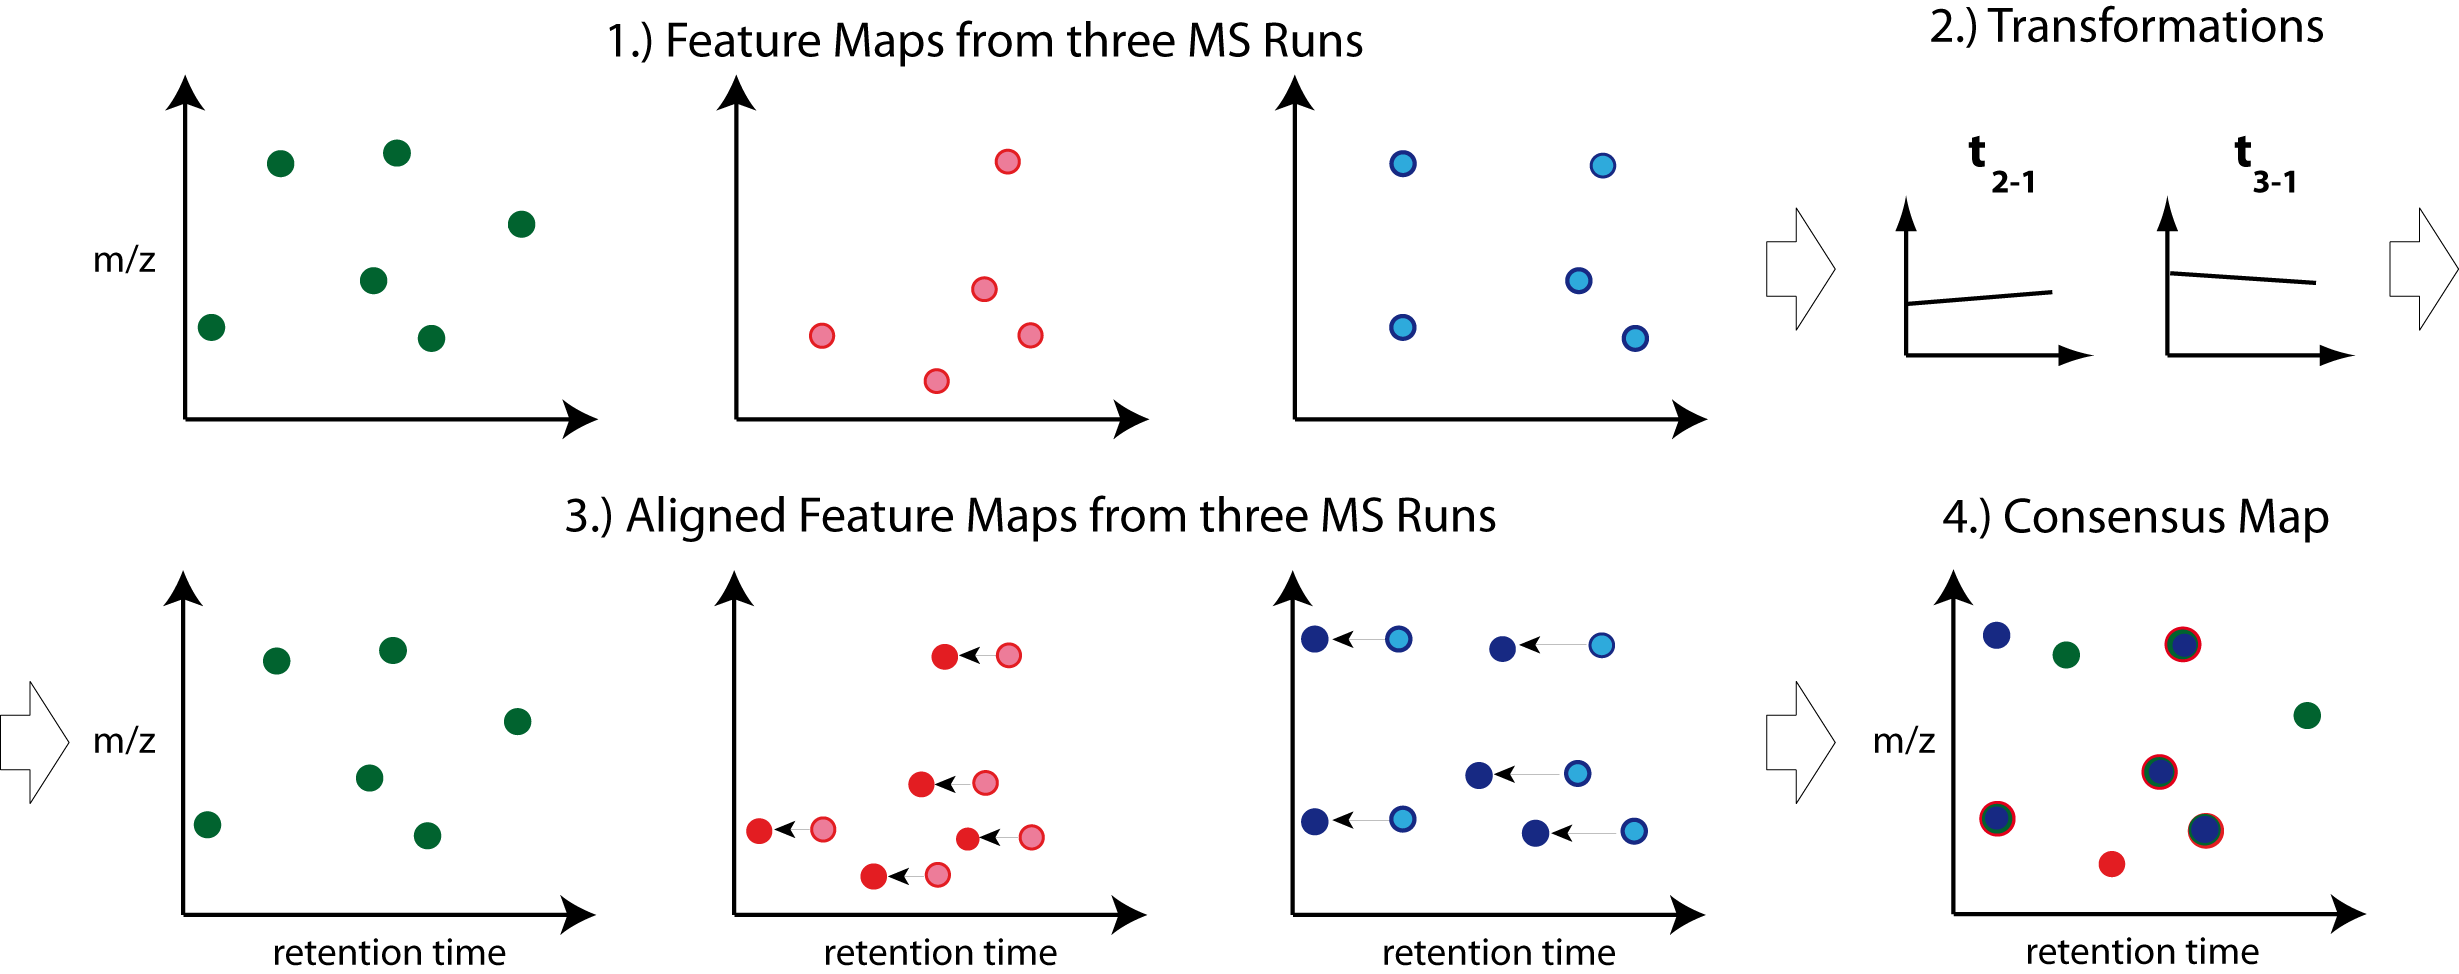
\includegraphics[width=\textwidth]{graphics/metabo/align.png}
	\caption[Map alignment]
	{
	\textbf{Map alignment.} The first feature map is used as a reference to which other maps are aligned. The calculated transformation brings corresponding features into close retention time proximity. Linking of these features form a so-called consensus features of a \textit{consensus map}.
	}
	\label{bg_alignment}
\end{figure}

\begin{itemize}
\item
After the \KNIMENODE{ZipLoopEnd} node add a \KNIMENODE{MapAlignerPoseClustering} node (\menu{Community Nodes > OpenMS > Map Alignment}), set its Output Type to featureXML, and adjust the following settings

\begin{center}
\begin{tabular}{l|l}
\textbf{parameter} & \textbf{value} \\ \hline
\textit{algorithm $\rightarrow$ max\_num\_peaks\_considered} & $-1$ \\
\textit{algorithm $\rightarrow$ superimposer $\rightarrow$ mz\_pair\_max\_distance} & $0.005$ \\
\textit{algorithm $\rightarrow$ superimposer $\rightarrow$ num\_used\_points} & $10000$ \\
\textit{algorithm $\rightarrow$ pairfinder $\rightarrow$ distance\_RT $\rightarrow$ max\_difference} & $20.0$ \\
\textit{algorithm $\rightarrow$ pairfinder $\rightarrow$ distance\_MZ $\rightarrow$ max\_difference} & $20.0$ \\
\textit{algorithm $\rightarrow$ pairfinder $\rightarrow$ distance\_MZ $\rightarrow$ unit} & ppm
\end{tabular}
\end{center}

\end{itemize}

\noindent \KNIMENODE{MapAlignerPoseClustering} provides an algorithm to align the retention time scales of multiple input files, correcting shifts and distortions between them. Retention time adjustment may be necessary to correct for chromatography differences e.g. before data from multiple LC-MS runs can be combined (feature linking). The alignment algorithm implemented here is the pose clustering algorithm. \\

\noindent The parameters change the behavior of \KNIMENODE{MapAlignerPoseClustering} as follows:
\begin{itemize}
\item \textbf{max\_num\_peaks\_considered}: The maximal number of peaks/features to be considered per map. To use all, set this parameter to -1.
\item \textbf{mz\_pair\_max\_distance}: Maximum of m/z deviation of corresponding elements in different maps.  This condition applies to the pairs considered in hashing.
\item \textbf{num\_used\_points}: Maximum number of elements considered in each map (selected by intensity). Use a smaller number to reduce the running time and to disregard weak signals during alignment.
\item \textbf{distance\_RT $\rightarrow$ max\_difference}: Features that have a larger RT difference will never be paired.
\item \textbf{distance\_MZ $\rightarrow$ max\_difference}: Features that have a larger m/z difference will never be paired.
\item \textbf{distance\_MZ $\rightarrow$ unit}: Unit used for the parameter distance\_MZ max\_difference, either Da or ppm.
\end{itemize}

The next step after retention time correction is the grouping of corresponding features in multiple samples. In contrast to the previous alignment, we assume no linear relations of features across samples. The used method is tolerant against local swaps in elution order.

\begin{figure}[htb]
	\centering
	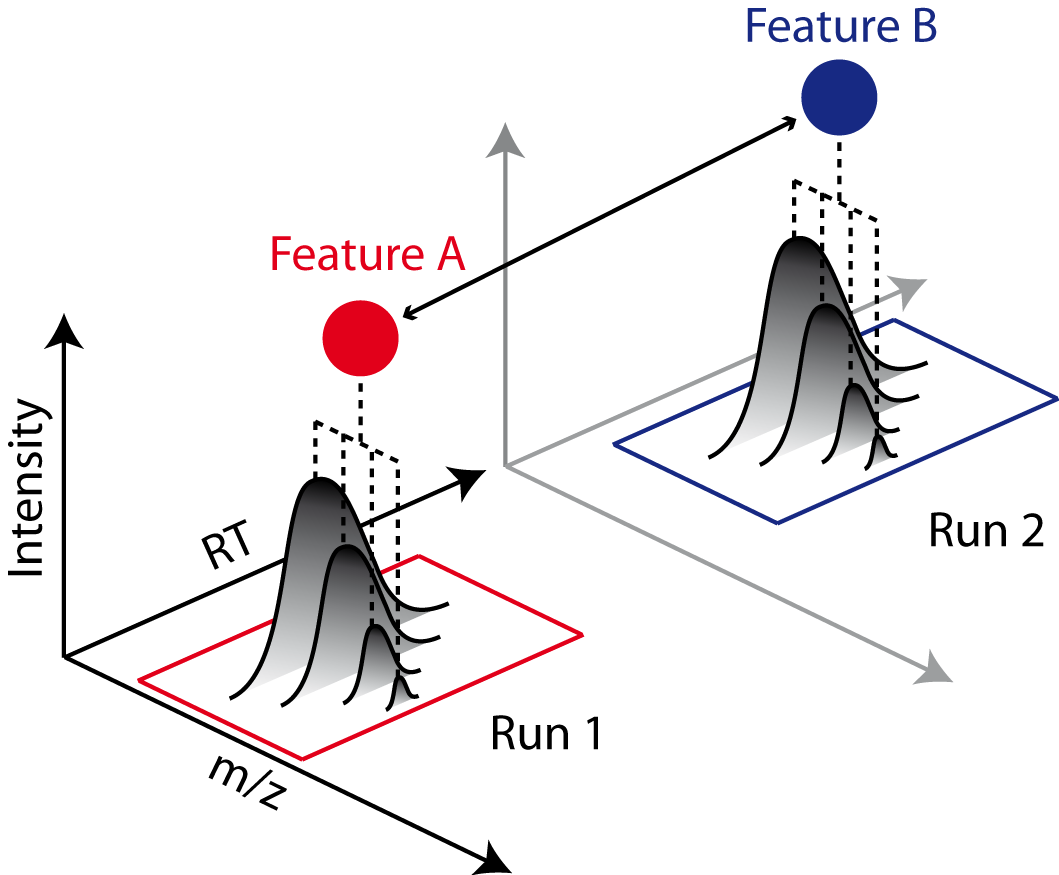
\includegraphics[width=0.7\textwidth]{graphics/metabo/link.png}
	\caption[Label-free quantification]
	{
	\textbf{Feature linking}. Features A and B correspond to the same analyte. The linking of features between runs (indicated by an arrow) allows comparing feature intensities.
	}
	\label{fig_bg_link}
\end{figure}

\begin{itemize}
\item
After the \KNIMENODE{MapAlignerPoseClustering} add a \KNIMENODE{FeatureLinkerUnlabeledQT} \\
 (\menu{Community Nodes > OpenMS > Map Alignment}) and adjust the following settings

\begin{center}
\begin{tabular}{l|l}
\textbf{parameter} & \textbf{value} \\ \hline
\textit{algorithm $\rightarrow$ distance\_RT $\rightarrow$ max\_difference} & $40.0$ \\
\textit{algorithm $\rightarrow$ distance\_MZ $\rightarrow$ max\_difference} & $20.0$ \\
\textit{algorithm $\rightarrow$ distance\_MZ $\rightarrow$ unit} & ppm
\end{tabular}
\end{center}

\noindent The parameters change the behavior of \KNIMENODE{FeatureLinkerUnlabeledQT} as follows (similar to the parameters we adjusted for \KNIMENODE{MapAlignerPoseClustering}):
\begin{itemize}
\item \textbf{distance\_RT $\rightarrow$ max\_difference}: Features that have a larger RT difference will never be paired.
\item \textbf{distance\_MZ $\rightarrow$ max\_difference}: Features that have a larger m/z difference will never be paired.
\item \textbf{distance\_MZ $\rightarrow$ unit}: Unit used for the parameter distance\_MZ max\_difference, either Da or ppm.
\end{itemize}

\item
After the \KNIMENODE{FeatureLinkerUnlabeledQT} add a \KNIMENODE{TextExporter} node (\menu{Community Nodes > OpenMS > File Handling}).
\item
Add an \KNIMENODE{Output Folder} node and configure it with an output directory where you want to store the resulting files.
\item
Run the pipeline and inspect the output.
\end{itemize}

\begin{figure}[htbp]
  \centering
  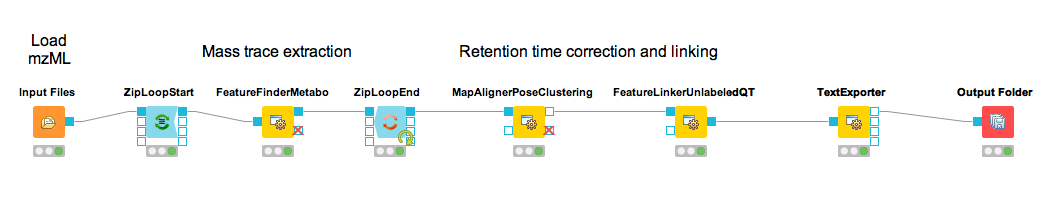
\includegraphics[width=0.85\textwidth]{graphics/metabo/metabo_part1_with_labels.png}
  \caption{Label-free quantification workflow for metabolites}
  \label{fig:metabo_part1}
\end{figure}

You should find a single, tab-separated file containing the information on where metabolites were found and with which intensities.
You can also add \KNIMENODE{Output Folder} nodes at different stages of the workflow and inspect the intermediate results (e.g., identified metabolite features for each input map).
The complete workflow can be seen in \cref{fig:metabo_part1}.
In the following section we will try to identify those metabolites.

\noindent The \KNIMENODE{FeatureLinkerUnlabeledQT} output can be visualized in ToppView on top of the input and output of the \KNIMENODE{FeatureFinderMetabo} (see Fig~\ref{fig:ToppView_5}). 

\begin{figure}[htbp]
  \centering
  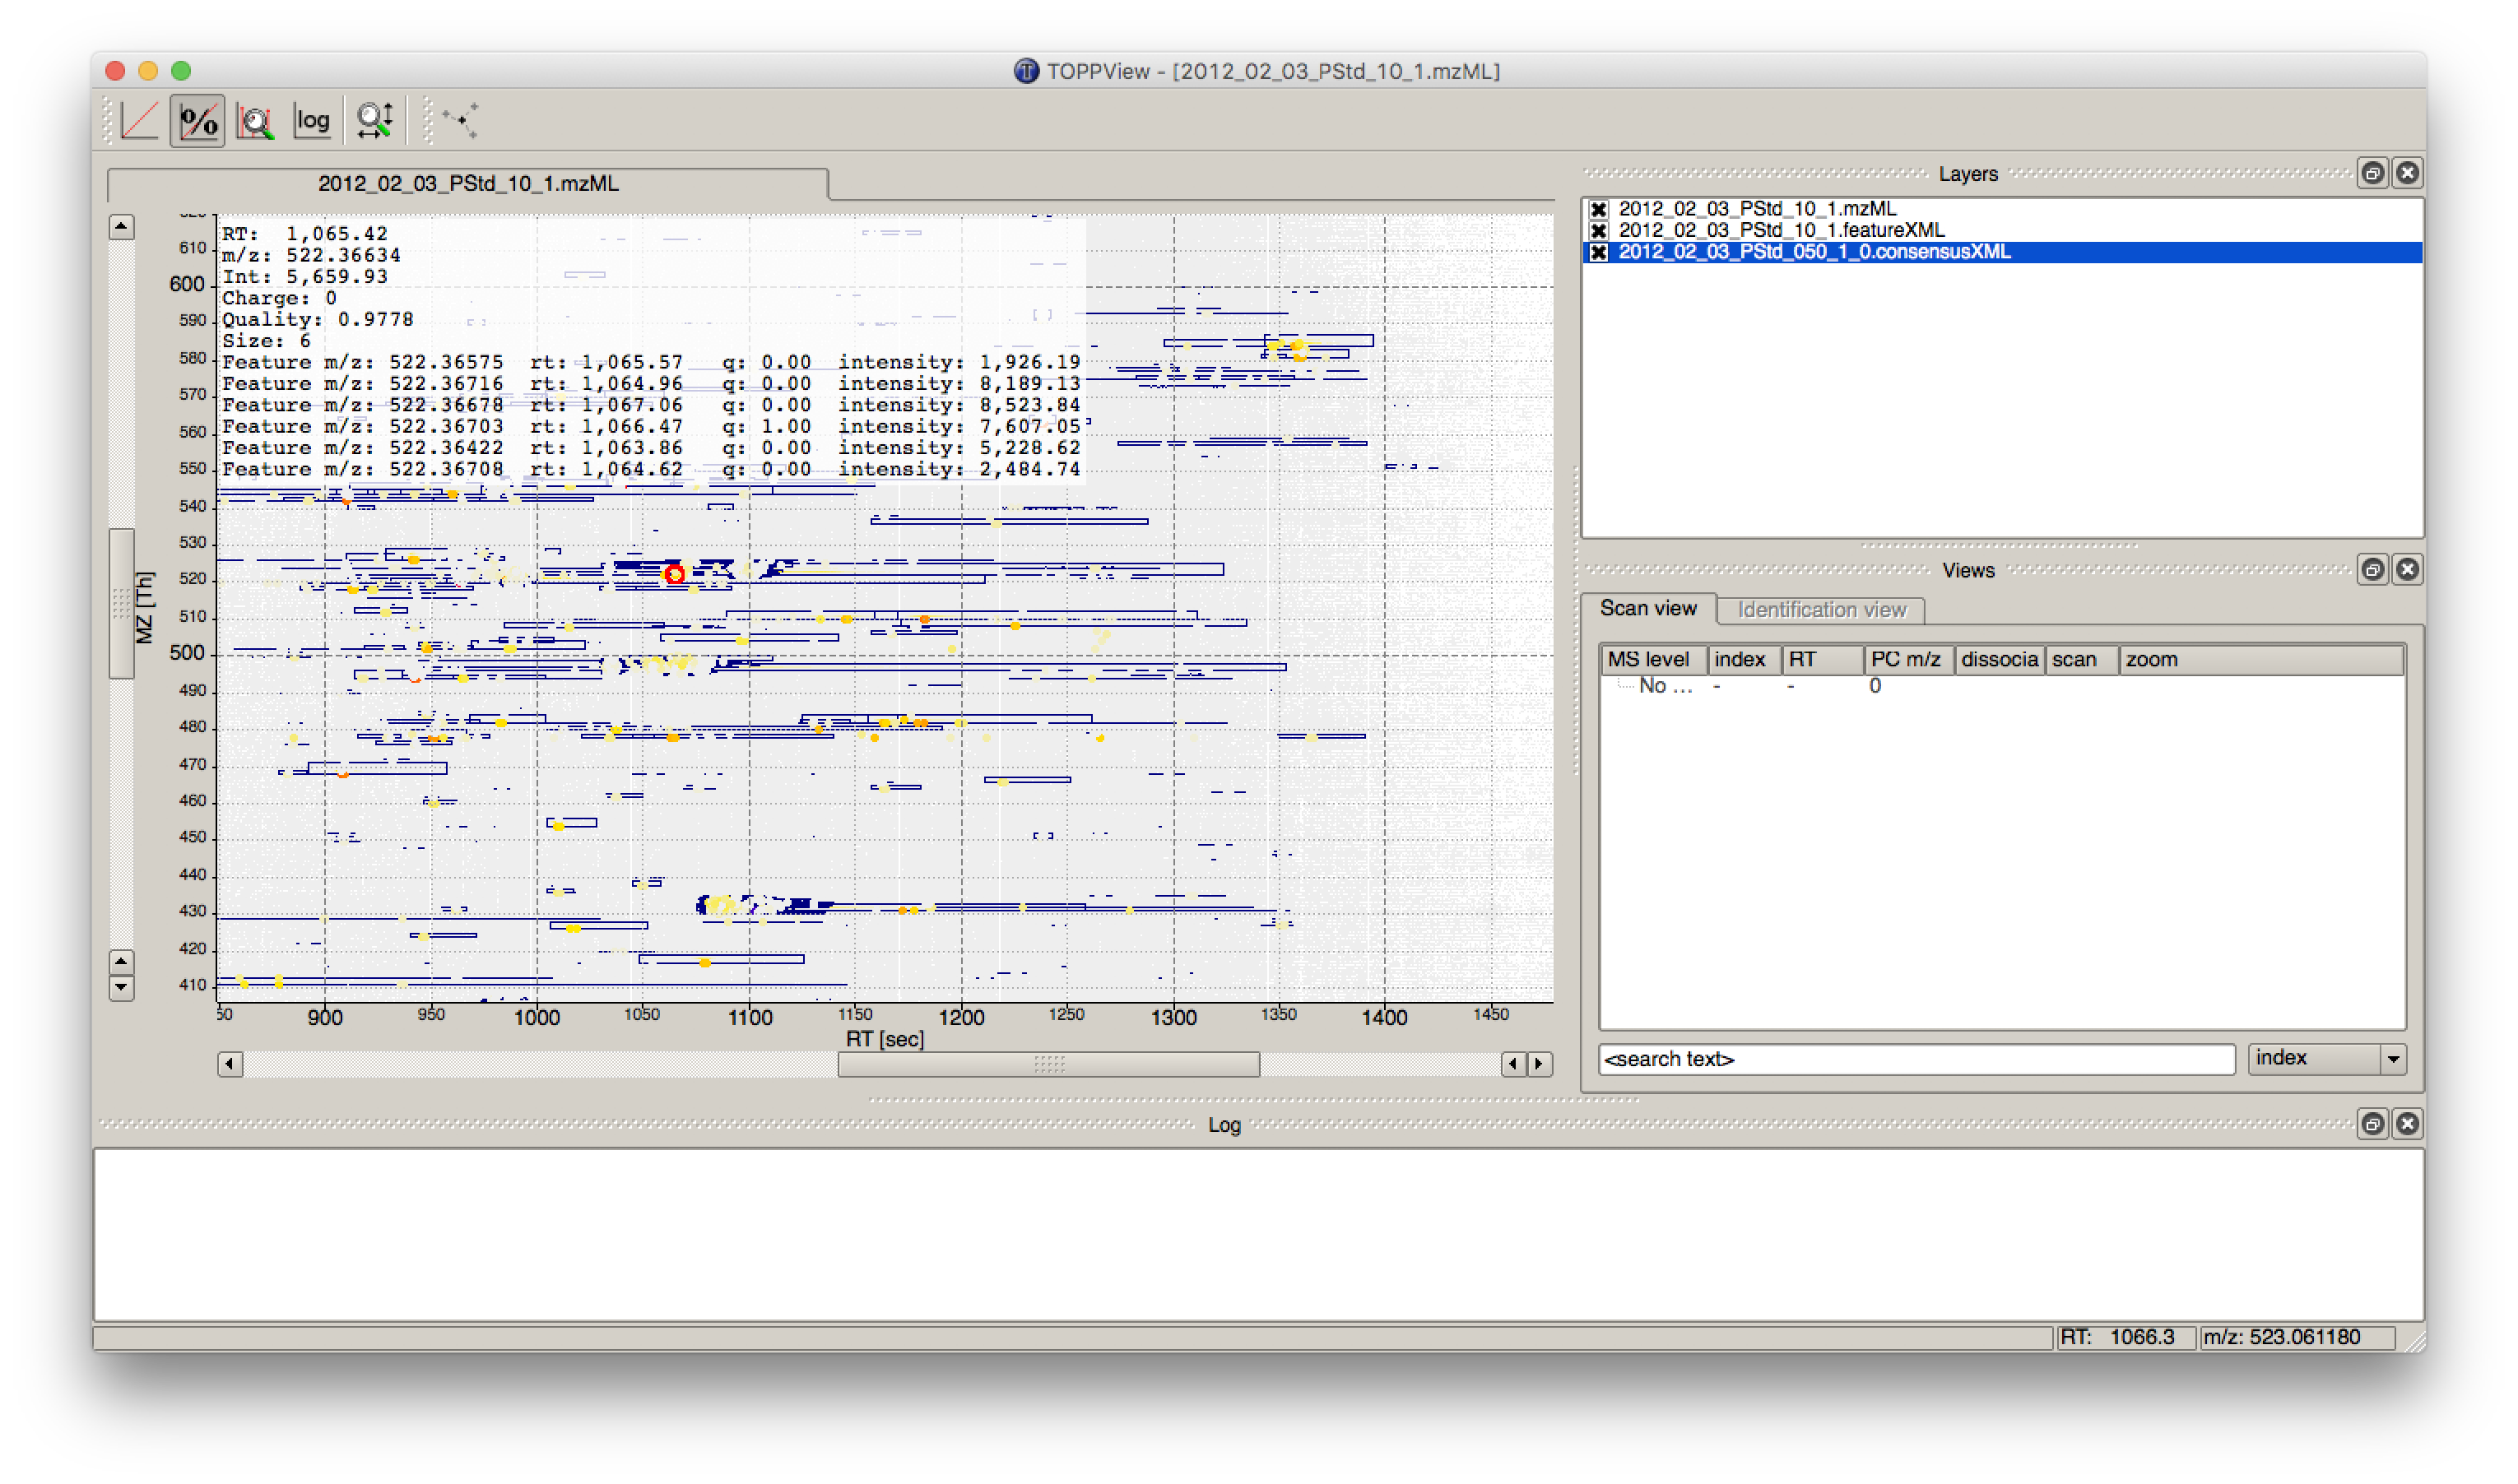
\includegraphics[width=\textwidth]{graphics/metabo/ToppView_5.png}
  \caption{Visualization of .consensusXML output over the .mzML and .featureXML 'layer'. }
  \label{fig:ToppView_5}
\end{figure}

\subsection{Basic metabolite identification}

At the current state we found several metabolites in the individual maps but so far don't know what they are.
To identify metabolites OpenMS provides multiple tools, including search by mass: the \KNIMENODE{AccurateMassSearch} node searches observed masses against the Human Metabolome Database (HMDB)\cite{Wishart2007,Wishart2009,Wishart2013}.
We start with the workflow from the previous section (see \cref{fig:metabo_part1}).

\begin{itemize}
\item
Add a \KNIMENODE{FileConverter} node (\menu{Community Nodes > OpenMS > File Handling}) and connect the output of the \KNIMENODE{FeatureLinkerUnlabeledQT} to the incoming port.
\item
Open the Configure dialog of the \KNIMENODE{FileConverter} and select the tab "OutputTypes".
In the drop down list for FileConverter.1.out select "featureXML".
\item
Add an \KNIMENODE{AccurateMassSearch} node (\menu{Community Nodes > OpenMS > Utilities}) and connect the output of the \KNIMENODE{FileConverter} to the first port of the \KNIMENODE{AccurateMassSearch}.
\item
Add four \KNIMENODE{Input File} nodes and configure them with the following files
\begin{itemize}
\item
\directory{Example\_Data / Metabolomics / databases / PositiveAdducts.tsv}\\
This file specifies the list of adducts that are considered in the positive mode. Each line contains the formula and charge of an adduct separated by a semicolon (e.g. M+H;1+). The mass of the adduct is calculated automatically.
\item
\directory{Example\_Data / Metabolomics / databases / NegativeAdducts.tsv}\\
This file specifies the list of adducts that are considered in the negative mode analogous to the positive mode.
\item
\directory{Example\_Data / Metabolomics / databases / HMDBMappingFile.tsv}\\
This file contains information from a metabolite database in this case from HMDB. It has three (or more) tab-separated columns: mass, formula, and identifier(s). This allows for an efficient search by mass.
\item
\directory{Example\_Data / Metabolomics / databases / HMDB2StructMapping.tsv}\\
This file contains additional information about the identifiers in the mapping file. It has four tab-separated columns that contain the identifier, name, SMILES, and INCHI. These will be included in the result file. The identifiers in this file must match the identifiers in the HMDBMappingFile.tsv.
\end{itemize}
\item
In the same order as they are given above connect them to the remaining input ports of the \KNIMENODE{AccurateMassSearch} node.
\item
Add an \KNIMENODE{Output Folder} node and connect the first output port of the \\
\KNIMENODE{AccurateMassSearch} node to the \KNIMENODE{Output Folder}.
\end{itemize}

The result of the \KNIMENODE{AccurateMassSearch} node is in the mzTab format \cite{Griss2014} so you can easily open it in a text editor or import it into Excel or KNIME, which we will do in the next section.
The complete workflow from this section is shown in \cref{fig:metabo_part2}.

\begin{figure}[htbp]
  \centering
  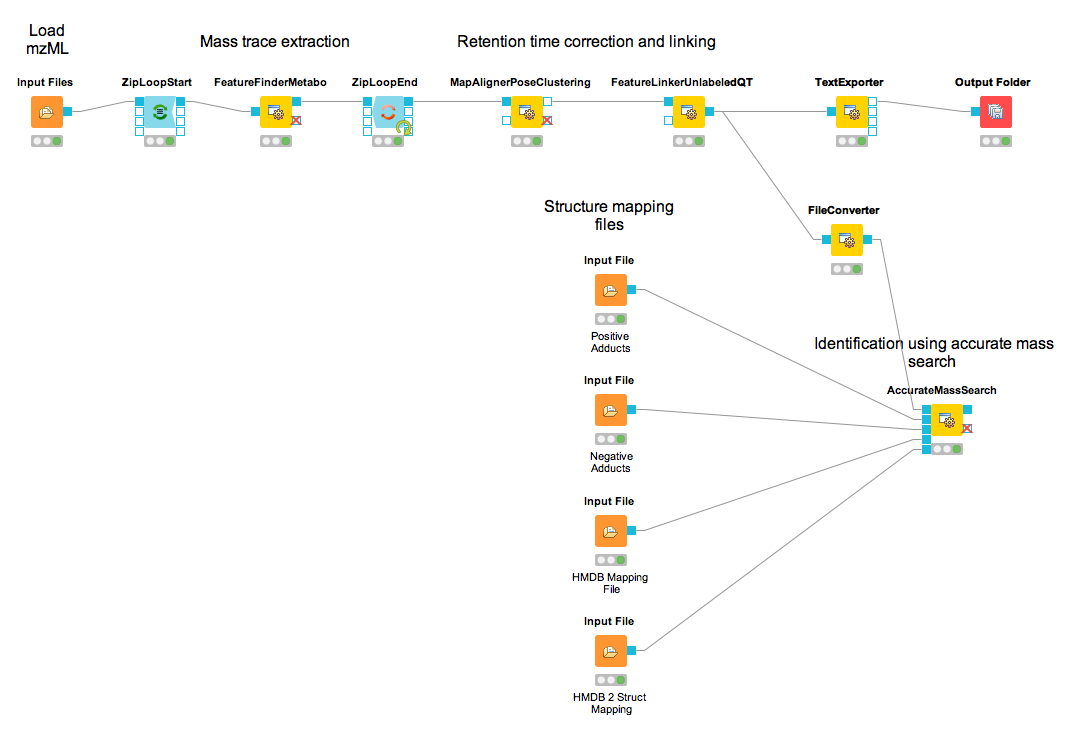
\includegraphics[width=0.85\textwidth]{graphics/metabo/metabo_part2.png}
  \caption{Label-free quantification and identification workflow for metabolites}
  \label{fig:metabo_part2}
\end{figure}

\subsubsection{Convert your data into a KNIME table}

The result from the \KNIMENODE{TextExporter} node as well as the result from the \KNIMENODE{AccurateMassSearch} node are files while standard KNIME nodes display and process only KNIME tables. To convert these files into KNIME tables we need two different nodes.
For the \KNIMENODE{AccurateMassSearch} results we use the \KNIMENODE{MzTabReader} node (\menu{Community Nodes > OpenMS > Conversion > mzTab}) and its \textit{Small Molecule Section} port. For the result of the \KNIMENODE{TextExporter} we use the \KNIMENODE{ConsensusTextReader} (\menu{Community Nodes > OpenMS > Conversion}).

When executed, both nodes will import the OpenMS files and provide access to the data as KNIME tables.
You can now easily combine both tables using the \KNIMENODE{Joiner} node (\menu{Manipulation > Column > Split \& Combine}) and configure it to match the m/z and retention time values of the respective tables.
The full workflow is shown in \cref{fig:metabo_part3}.

\begin{figure}[htbp]
  \centering
  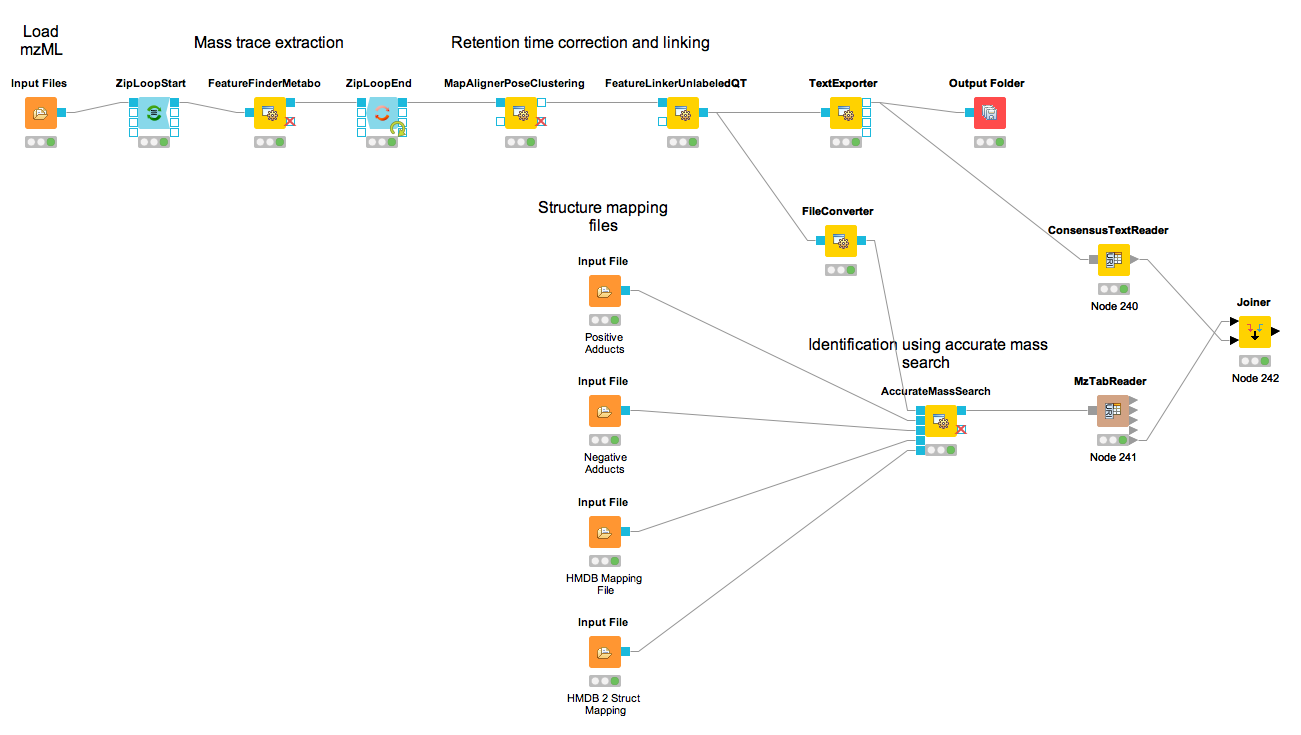
\includegraphics[width=0.85\textwidth]{graphics/metabo/metabo_part3.png}
  \caption{Label-free quantification and identification workflow for metabolites that loads the results into KNIME and joins the tables.}
  \label{fig:metabo_part3}
\end{figure}

\subsubsection{Visualizing data}

Now that you have your data in KNIME you should try to get a feeling for the capabilities of KNIME.

\begin{task}
Check out the \KNIMENODE{Molecule Type Cast}  node (\menu{Chemistry > Translators}) together with subsequent cheminformatics nodes (e.g. \KNIMENODE{RDKit From Molecule} (\menu{Community Nodes > RDKit > Converters})) to render the structural formula contained in the result table.

\end{task}
\begin{task}
Have a look at the \KNIMENODE{Column Filter} node to reduce the table to the interesting columns, e.g., only the Ids, chemical formula, and intensities.
\end{task}
\begin{task}
Try to compute and visualize the m/z and retention time error of the different feature elements (from the input maps) of each consensus feature. Hint: A nicely configured \KNIMENODE{Math Formula (Multi Column)} node should suffice.
\end{task}

\subsubsection{Spectral library search}

Identifying metabolites using only the accurate mass may lead to ambiguous results. In practice, additional information (e.g. the retention time) is used to further narrow down potential candidates. Apart from MS1-based features, tandem mass spectra (MS2) of metabolites provide additional information.
In this part of the tutorial, we take a look on how metabolite spectra can be identified using a library of previously identified spectra.

\noindent Because these libraries tend to be large we don't distribute them with OpenMS. 

\begin{task}
Construct the workflow as shown in Fig.~\ref{fig:speclib}.
Use the file \directory{Example\_Data / Metabolomics / datasets \newline / Metabolite\_ID\_SpectraDB\_positive.mzML} as input for your workflow.  You can use the spectral library from \\
\directory{Example\_Data / Metabolomics / databases / MetaboliteSpectralDB.mzML}\\ as second input. 
The first input file contains tandem spectra that are identified by the \KNIMENODE{MetaboliteSpectralMatcher}. The resulting mzTab file is read back into a KNIME table and stored in an Excel table. Make sure that you connect the MzTabReader port corresponding to the Small Molecule Section to the \KNIMENODE{Excel writer (XLS)}. Please select the "add column headers" option in the \KNIMENODE{Excel writer (XLS)}).

\end{task}

\begin{figure}[htbp]
  \centering
  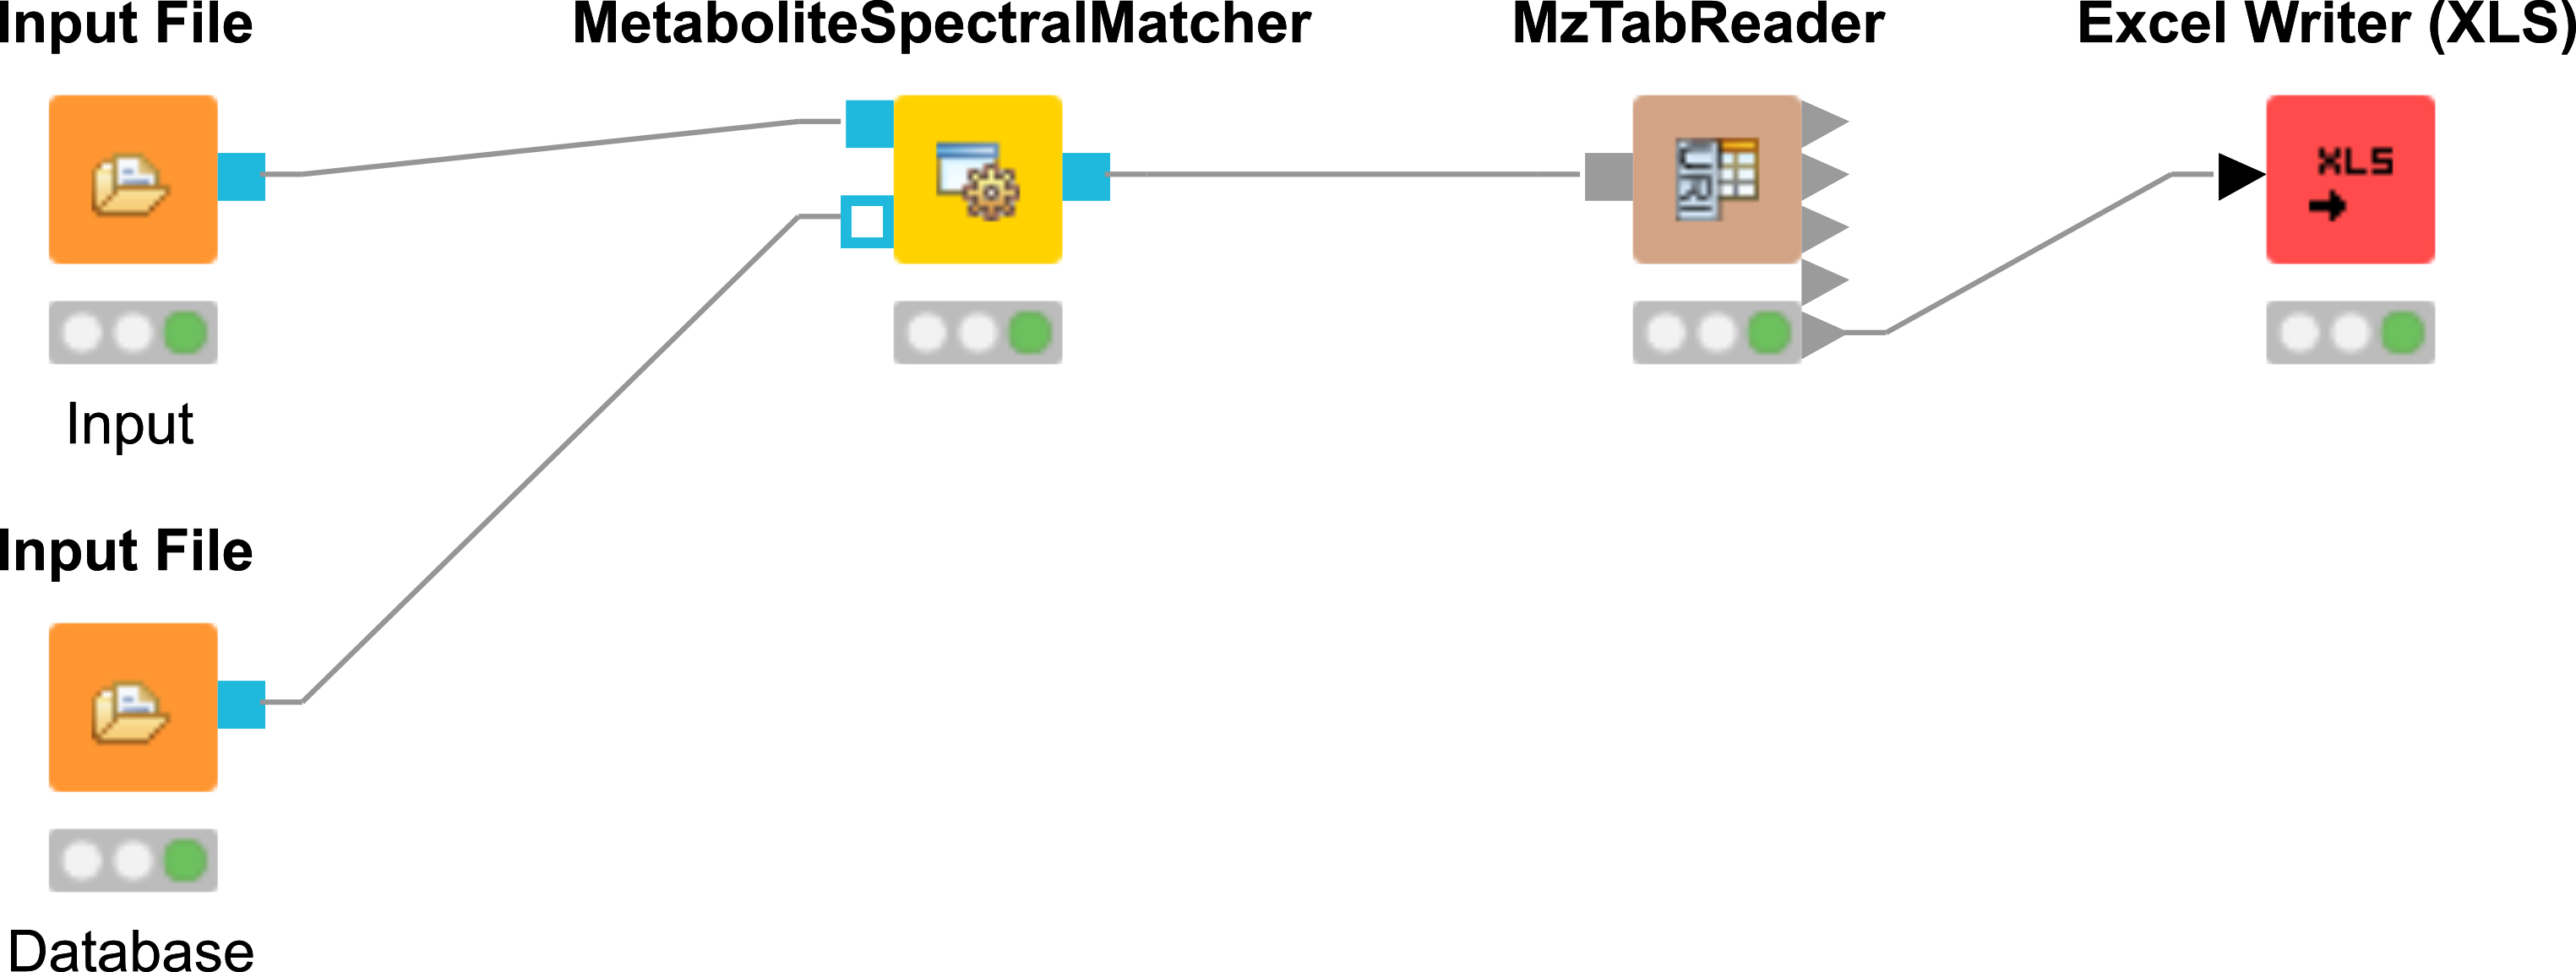
\includegraphics[width=0.7\textwidth]{graphics/metabo/speclib.png}
  \caption{Spectral library identification workflow}
  \label{fig:speclib}
\end{figure}

Run the workflow and inspect the output.

\subsubsection{Manual validation}

In metabolomics, matches between tandem spectra and spectral libraries are manually validated. Several commercial and free online resources exist which help in that task. Some examples are:

\begin{itemize}
\item mzCloud contains only spectra from Thermo Orbitrap instruments. The webpage requires Microsoft Silverlight which currently does not work in modern browsers (see \url{https://www.mzcloud.org/DataViewer}).
\item MassBank North America (MoNA) has spectra from different instruments but falls short in in number of spectra (compared to Metlin and mzCloud) \url{http://mona.fiehnlab.ucdavis.edu/spectra/display/KNA00122}
\item METLIN includes 961,829 molecules ranging from lipids, steroids, metabolites, small peptides, carbohydrates, exogenous drugs and toxicants. In total over 14,000 metabolites.
\end{itemize}

Here, we will use METLIN to manually validate metabolites.

\begin{task}
Check in the .xlsx output from the \KNIMENODE{Excel writer (XLS)} if you can find glutathione. Use the retention time column to find the spectrum in the mzML file. Here open the file in the \directory{Example\_Data / Metabolomics / datasets \newline / Metabolite\_ID\_SpectraDB\_positive.mzML} in  TOPPView. The MSMS spectrum with the retention time of 67.6 s is used as example. The spectrum can be selected based on the retention time in the scan view window. Therefore the MS1 spectrum with the retention time of 66.9 s has to be double clicked and the MSMS spectra recorded in this time frame will show up. Select the tandem spectrum of Glutathione, but do not close TOPPView, yet.
\end{task} 

\begin{figure}[htbp]
  \centering
  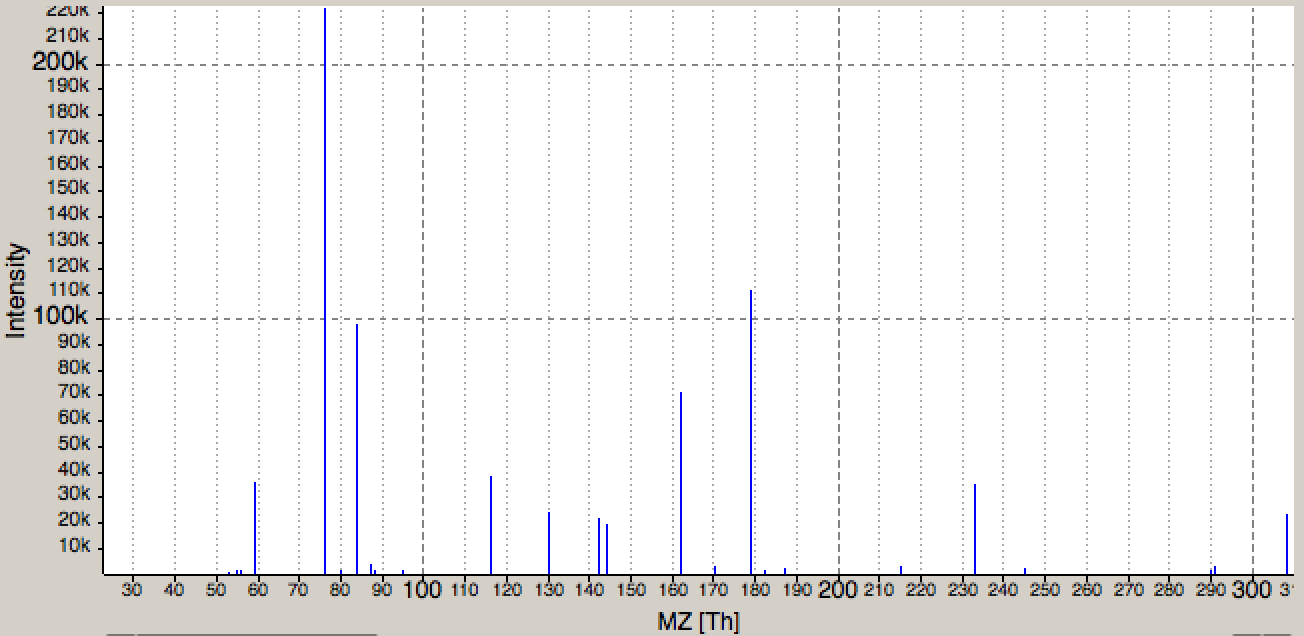
\includegraphics[width=0.85\textwidth]{graphics/metabo/glutathioneTV.png}
  \caption{Tandem spectrum of glutathione. Visualized in TOPPView.}
  \label{fig:glutathioneTandemSpectrum}
\end{figure}

\begin{task}
On the METLIN homepage search for \menu{Compound Name} Glutathione using the \menu{Advanced Search} (\url{https://metlin.scripps.edu/landing_page.php?pgcontent=advanced_search}). Note that free registration is required. Which collision energy (and polarity) gives the best (visual) match to your experimental spectrum in TOPPView? Here you can compare the fragmentation patterns in both spectra shown by the Intensity or relative Intensity, the m/z of a peak and the distance between peaks. Each distance between two peaks corresponds to a fragment of elemental composition (e.g., NH2 with the charge of one would have mass of two peaks of 16.023 Th).
\end{task}

\begin{figure}[htbp]
  \centering
  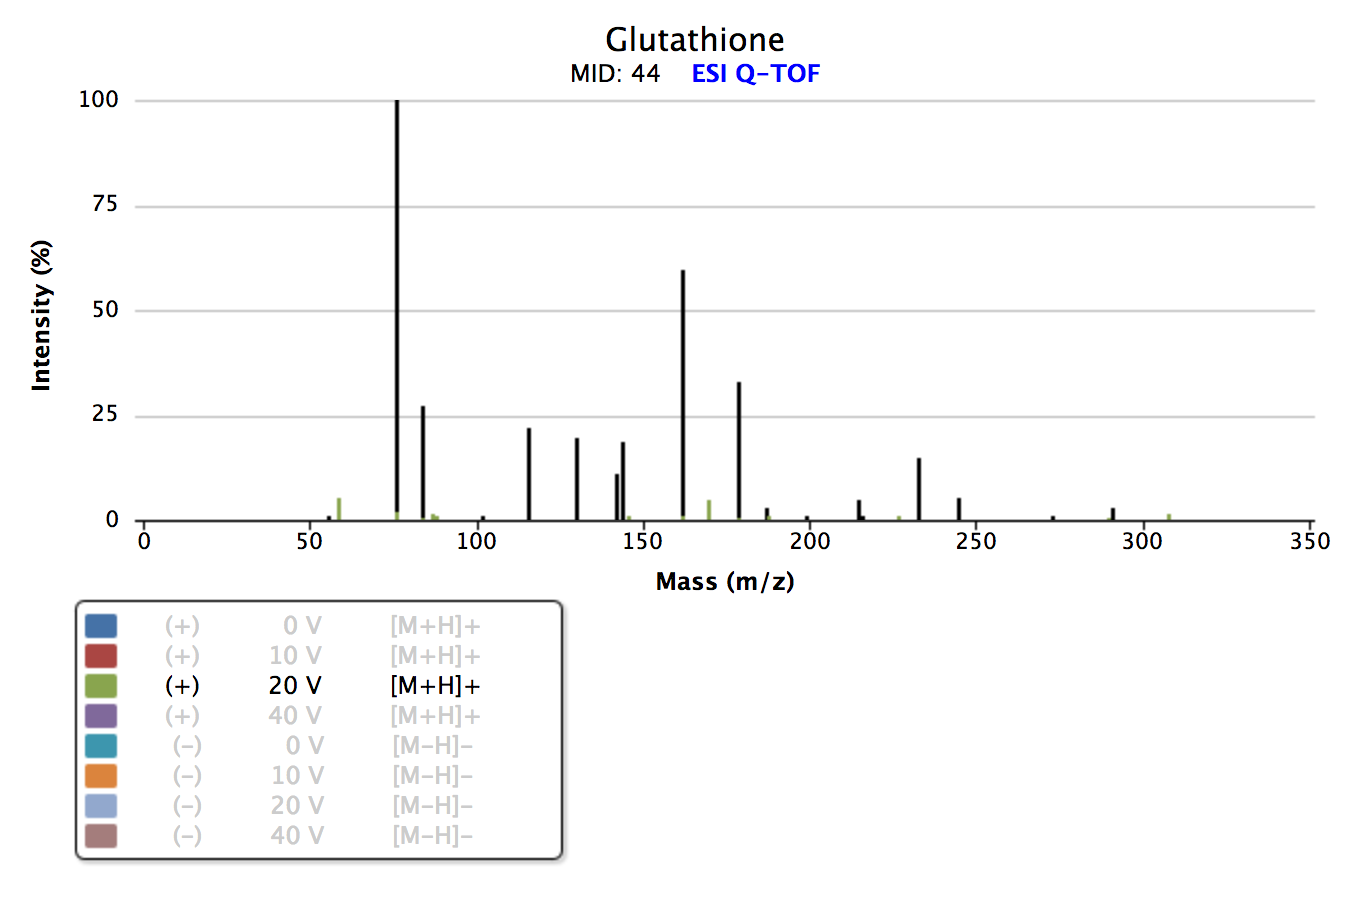
\includegraphics[width=0.85\textwidth]{graphics/metabo/glutathioneMetlin.png}
  \caption{Tandem spectrum of glutathione. Visualized in Metlin. Note that several fragment spectra from varying collision energies are available.}
  \label{fig:glutathioneMetlin}
\end{figure}

\subsubsection{De novo identification}

Another method for identification of metabolites using the MS2 spectra is de-novo identification. 
This can be used in addition to the other methods (accurate mass search, spectral library search) or individually if no spectral spectral library is available. In this part of the tutorial, we take a look on how metabolite spectra can be identified using de-novo tools. To this end, the tool SIRIUS and CSI:FingerID (\cite{Bocker2009,Bocker2016,Duhrkop2015}) was integrated in the OpenMS Framework as SiriusAdapter. SIRIUS uses isotope pattern analysis for detecting the molecular formula and further analyses the fragmentation pattern of a compound using fragmentation treesCSI:FingerID  is a method for searching a tandem mass spectrum of a small molecule (metabolite) in a database of molecular structures.

The is able to work in different modes depending on the provided input. 
\begin{itemize}
\item Input: mzML - SiriusAdapter will use the MS1 and MS2 information provided and search all MS2 spectra in a map.  
\item Input: mzML, featureXML (FeatureFinderMetabo) - SiriusAdapter can use the provided feature information to reduce the search space to valid Features with MS2 spectra. Additional it can use the Isotope trace information. 
\item Input: mzML, featureXML (FeatureFinderMetabo and MetaboliteAdductDecharger) - SiriusAdapter can use the feature information as mentioned above. Further adduct information of the feature is provided by using adduct grouping. 
\end{itemize}

The last method is the preferred one, since SIRIUS gains a lot of additional information by using the OpenMS preprocessing. 

\begin{task}
Construct the workflow as shown in Fig.~\ref{fig:denovoid}. \\
Use the file \directory{Example\_Data / Metabolomics / datasets \newline / Metabolite\_DeNovoID\.mzML} as input for your workflow.  
\end{task}

\begin{figure}[htbp]
  \centering
  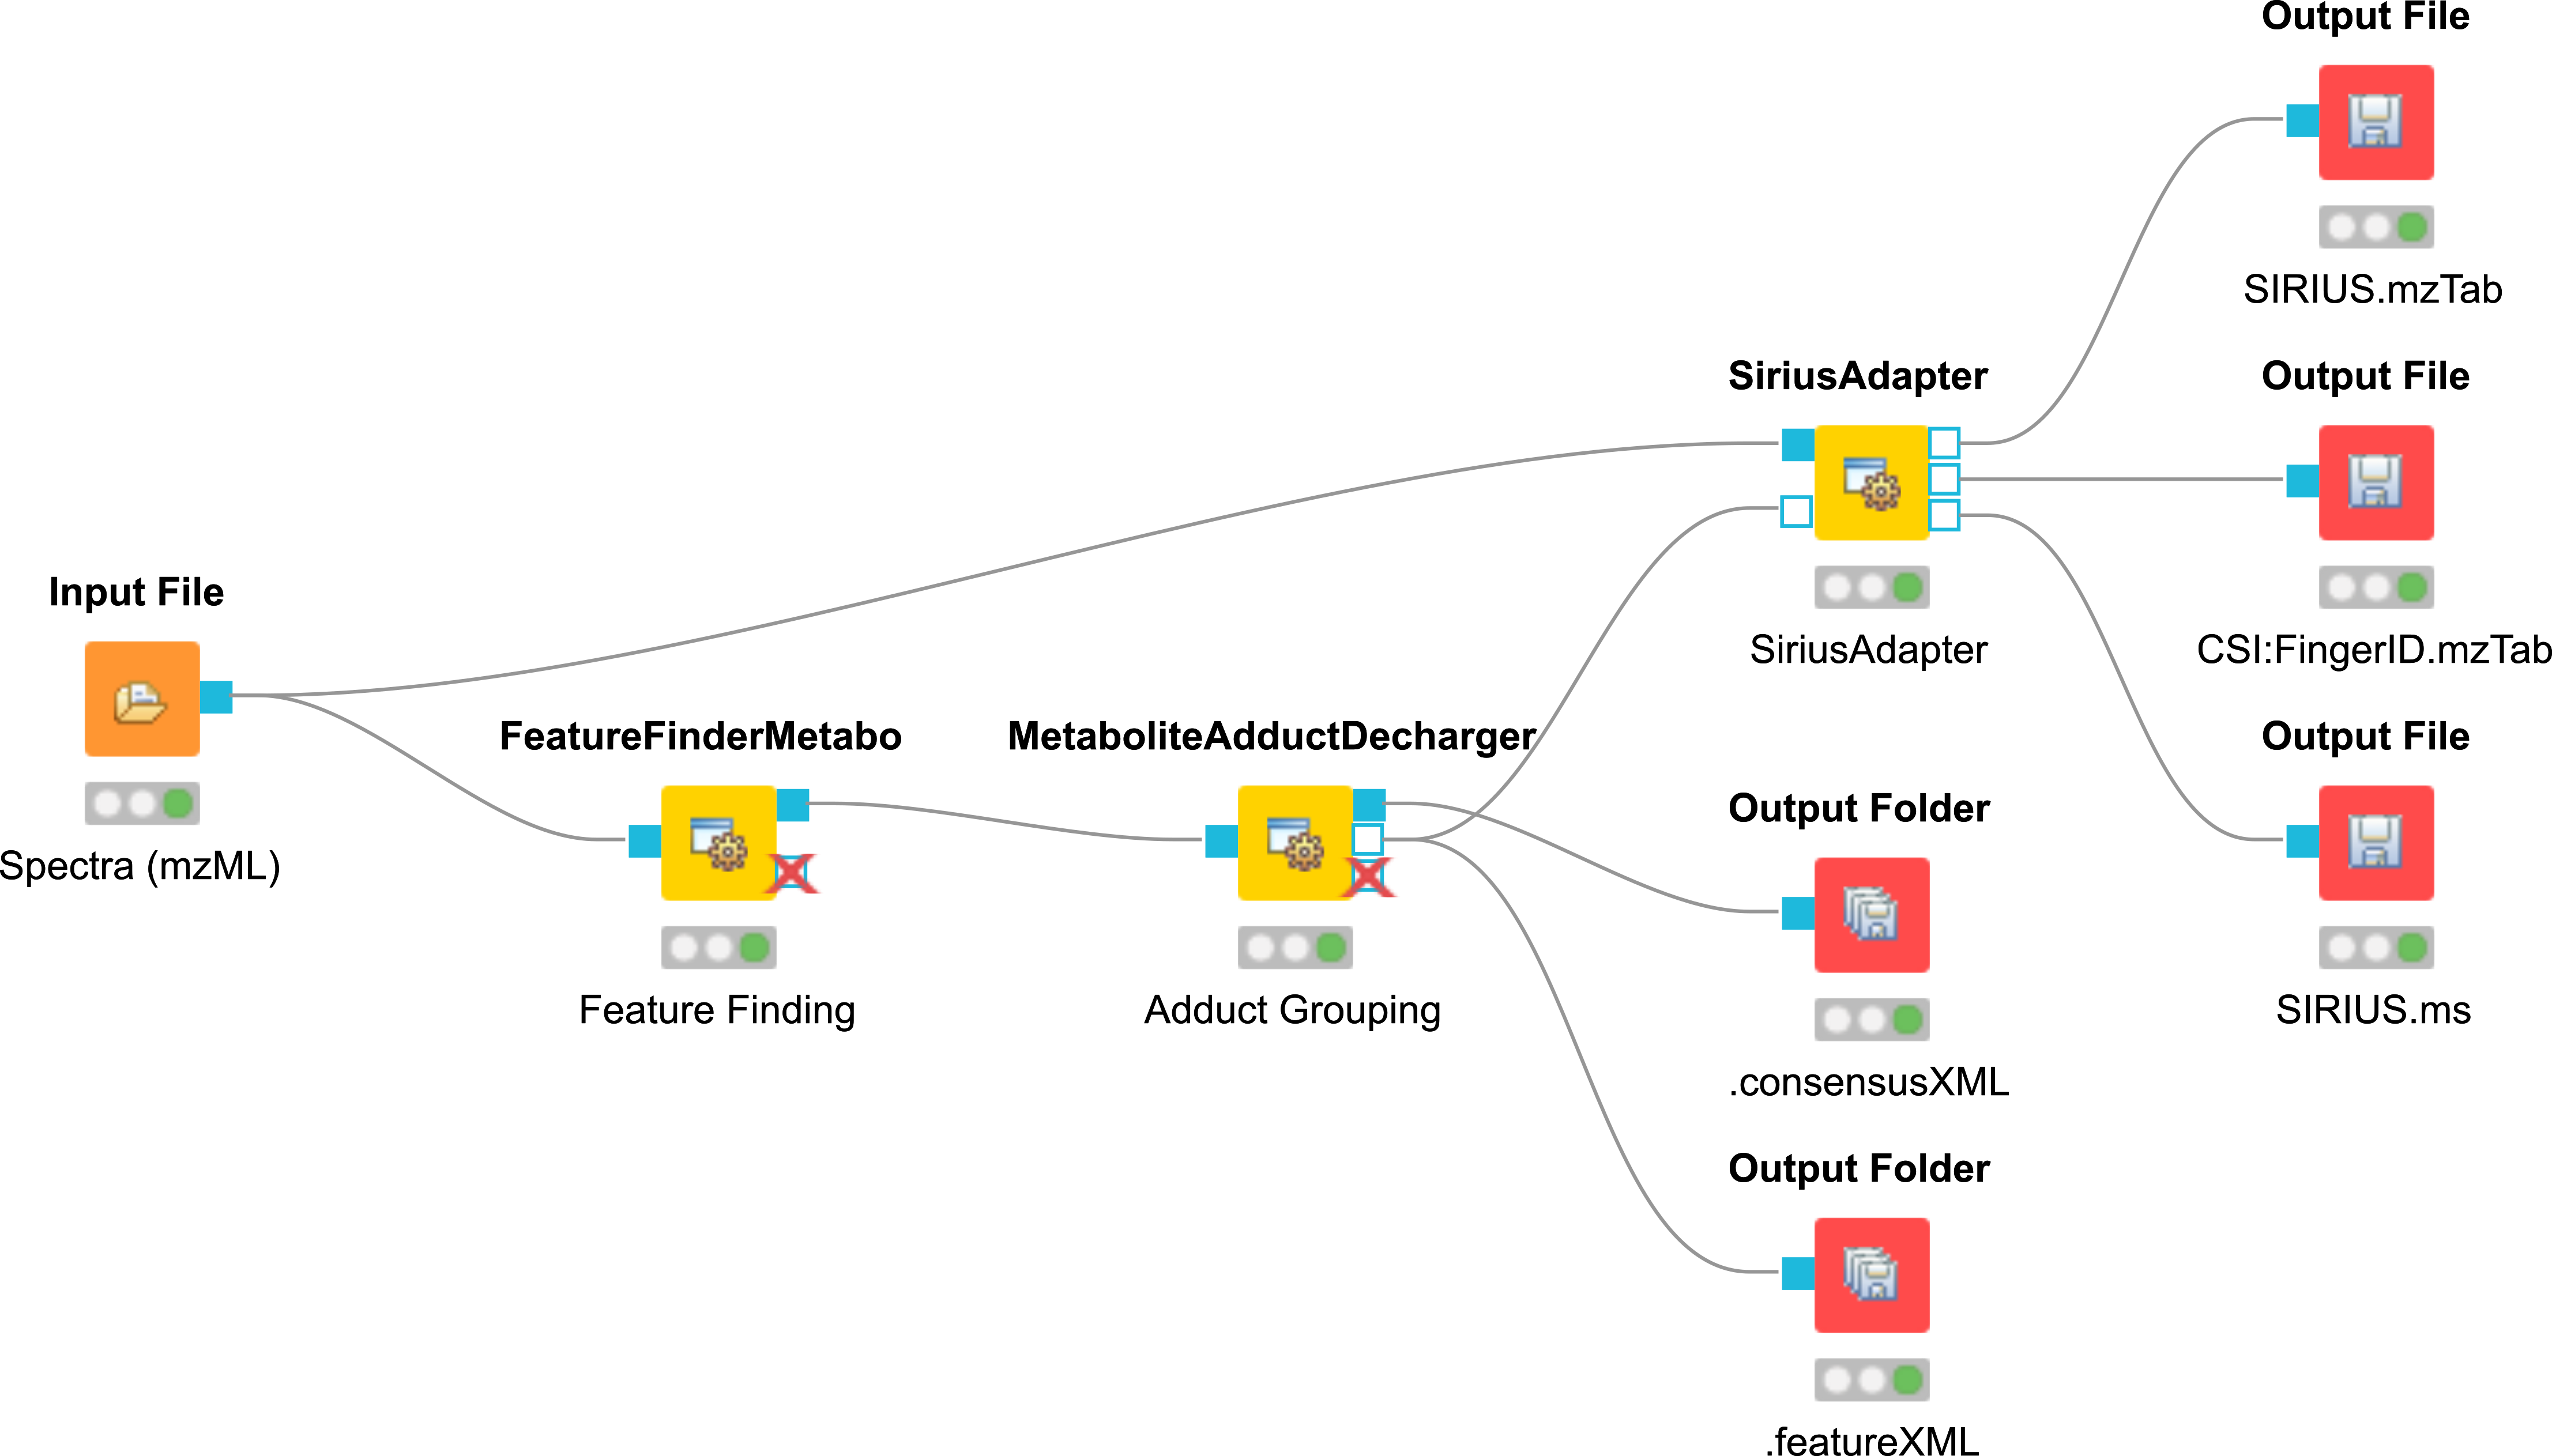
\includegraphics[width=0.85\textwidth]{graphics/metabo/denovoid.png}
  \caption{De novo identification workflow}
  \label{fig:denovoid}
\end{figure}

Run the workflow and inspect the output. \\

\noindent The output consists of two mzTab files . One for the SIRIUS and the other for the CSI:FingerID summary. These provide information about the sumformula, adduct and the possible compound structure. The information is referenced to the spectrum used in the analysis. Additional information can be extracted by using the \KNIMENODE{SiriusAdapter} debug output. Here the SIRIUS workspace will be provided after the calculation has finished. The folder contains information about annotated fragments for each successfully explained compound.  

The debug folder can be found by selecting the \KNIMENODE{SiriusAdapter} after the workflow has finished and using its \menu{View: SiriusAdapter Std Output}. Here the path found in \menu{Keeping temporary files in directory}can be copied to your file manger - this will be simplified in the next OpenMS release.

%%%%%%%%%%%%%%%%%%%%%%%%%%%%%%%%%%%%%%%%%%%%%%%%%%%%%%%%%%%%%%%%%%%%%%%%%%%%%%%%%%%%%%%%%%%%%%%%%%%%%%%%%%%%%%%%%%%%%%%%%%%%%%%%%%%%
\subsection{Downstream data analysis and reporting}
In this part of the metabolomics session we take a look at more advanced downstream analysis and the use of the statistical programming language R. As laid out in the introduction we try to detect a set of spike-in compounds against a complex blood background. As there are many ways to perform this type of analysis we provide a complete workflow.

\begin{task}
Import the workflow from \directory{Workflows / metabolite\_ID.knwf} in KNIME: \menu{File > Import KNIME Workflow...}
\end{task}

The section below will guide you in your understanding of the different parts of the workflow. Once you understood the workflow you should play around and be creative. Maybe create a novel visualization in KNIME or R? Do some more elaborate statistical analysis? Note that some basic R knowledge is required to fully understand the processing in \KNIMENODE{R Snippet} nodes.

\subsubsection{Signal processing and data preparation for identification}
This part is analogous to what you did for the simple metabolomics pipeline.

\subsubsection{Data preparation for quantification}
The first part is identical to what you did for the simple metabolomics pipeline. Additionally, we convert zero intensities into NA values and remove all rows that contain at least one NA value from the analysis. We do this using a very simple \KNIMENODE{R Snippet} and subsequent \KNIMENODE{Missing Value filter} node.

\begin{task}
Inspect the \KNIMENODE{R Snippet} by double-clicking on it. The KNIME table that is passed to an \KNIMENODE{R Snippet} node is available in R as a data.frame named knime.in. The result of this node will be read from the data.frame knime.out after the script finishes. Try to understand and evaluate parts of the script (Eval Selection). In this dialog you can also print intermediary results using for example the R command head(knime.in) or cat(knime.in) to the Console pane.
\end{task}

\subsubsection{Statistical analysis}
After we linked features across all maps, we want to identify features that are significantly deregulated between the two conditions. We will first scale and normalize the data, then perform a t-test, and finally correct the obtained p-values for multiple testing using Benjamini-Hochberg. All of these steps will be carried out in individual \KNIMENODE{R Snippet} nodes.
\begin{itemize}
\item Double-click on the first \KNIMENODE{R Snippet} node labeled "log scaling" to open the \KNIMENODE{R Snippet} dialog. In the middle you will see a short R script that performs the log scaling. To perform the log scaling we use a so-called regular expression (grepl) to select all columns containing the intensities in the six maps and take the $log_2$ logarithm.

\item The output of the log scaling node is also used to draw a boxplot that can be used to examine the structure of the data. Since we only want to plot the intensities in the different maps (and not m/z or rt) we first use a \KNIMENODE{Column Filter} node to keep only the columns that contain the intensities. We connect the resulting table to a \KNIMENODE{Box Plot} node which draws one box for every column in the input table. Right-click and select \menu{View: Box Plot}.

\item The median normalization is performed in a similar way to the log scaling. First we calculate the median intensity for each intensity column, then we subtract the median from every intensity.

\item Open the \KNIMENODE{Box Plot} connected to the normalization node and compare it to the box plot connected to the log scaling node to examine the effect of the median normalization.

\item To perform the t-test we defined the two groups we want to compare. Then we call the t-test for every consensus feature unless it has missing values. Finally we save the p-values and fold-changes in two new columns named p-value and FC.

\item The \KNIMENODE{Numeric Row Splitter} is used to filter less interesting parts of the data. In this case we only keep columns where the fold-change is $\geq$ 2.

\item We adjust the p-values for multiple testing using Benjamini-Hochberg and keep all consensus features with a q-value $\leq$ 0.01 (i.e. we target a false-discovery rate of $1\%$).

\end{itemize}


\subsubsection{Interactive visualization}

KNIME supports multiple nodes for interactive visualization with interrelated output. The nodes used in this part of the workflow exemplify this concept. They further demonstrate how 
figures with data dependent customization can be easily realized using basic KNIME nodes. Several simple operations are concatenated in order to enable an interactive volcano plot.
\begin{itemize}
\item We first log-transform fold changes and p-values in the \KNIMENODE{R Snippet} node. We then append columns noting interesting features (concerning fold change and p-value).
\item With this information, we can use various Manager nodes (\menu{Views > Property}) to emphasize interesting data points. The configuration dialogs allow us to select columns to change color, shape or size of data points dependent on the column values.
\item The \KNIMENODE{Scatter Plot} node (\menu{Views}) enables interactive visualization of the logarithmized values as a volcano plot: the log-transformed values can be chosen in the `Column Selection' tab of the plot view. Data points can be selected in the plot and HiLited via the menu option. HiLiteing transfers to all other interactive nodes connected to the same data table. In our case, selection and HiLiteing will also occur in the \KNIMENODE{Interactive Table} node (\menu{Views}).
\item Output of the interactive table can then be filtered via the HiLite menu tab. For example, we could restrict shown rows to points HiLited in the volcano plot.
\end{itemize}
\begin{task}
Inspect the nodes of this section. Customize your visualization and possibly try to visualize other aspects of your data.
\end{task}

\subsubsection{Advanced visualization}
\label{sec:metaboR}
R Dependencies: This section requires that the R packages \texttt{ggplot2} and \texttt{ggfortify} are both installed. \texttt{ggplot2} is part of the \textit{KNIME R Statistics Integration (Windows Binaries)} which should already be installed via the full KNIME installer, \texttt{ggfortify} however is not.
In case that you use an R installation where one or both of them are not yet installed, add an \KNIMENODE{R Snippet} node and double-click to configure. In the \textit{R Script} text editor, enter the following code:
\begin{lstlisting}
#Include the next line if you also have to install ggplot2:
install.packages("ggplot2")
#Include the following lines to install ggfortify:
install.packages("ggfortify")
library(ggplot2)
library(ggfortify)
\end{lstlisting}
You can remove the \texttt{install.packages} commands once it was successfully installed.

Even though the basic capabilities for (interactive) plots in KNIME are valuable for initial data exploration, professional looking depiction of analysis results often relies on dedicated plotting libraries. The statistics language R supports the addition of a large variety of packages, including packages providing extensive plotting capabilities. This part of the workflow shows how to use R nodes in KNIME to visualize more advanced figures. Specifically, we make use of different plotting packages to realize heatmaps.


\begin{itemize}
\item The used \KNIMENODE{RView (Table)} nodes combine the possibility to write R snippet code with visualization capabilities inside KNIME. Resulting images can be looked at in the output RView, or saved via the \KNIMENODE{Image Port Writer} node.
\item The heatmap nodes make use of the gplots libary, which is by default part of the R Windows binaries (for full KNIME version 3.1.1 or higher). We again use regular expressions to extract all measured intensity columns for plotting. For clarity, feature names are only shown in the heatmap after filtering by fold changes.
\end{itemize}

\subsubsection{Data preparation for Reporting}
Following the identification, quantification and statistical analysis our data is merged and formatted for reporting.
First we want to discard our normalized and logarithmized intensity values in favor of the original ones.
To this end we first remove the intensity columns (\KNIMENODE{Column Filter}) and add the original intensities back (\KNIMENODE{Joiner}).
For that we use an \textit{Inner Join} \footnote{\textit{Inner Join} is a technical term that describes how database tables are merged.} with the \KNIMENODE{Joiner} node. In the dialog of the node we add two entries for the Joining Columns and for the first column we pick "retention\_time" from the top input (i.e. the AccurateMassSearch output) and "rt\_cf" (the retention time of the consensus features) for the bottom input (the result from the quantification). For the second column you should choose "exp\_mass\_to\_charge" and "mz\_cf" respectively to make the joining unique. Note that the workflow needs to be executed up to the previous nodes for the possible selections of columns to appear.

\begin{figure}[htbp]
  \centering
  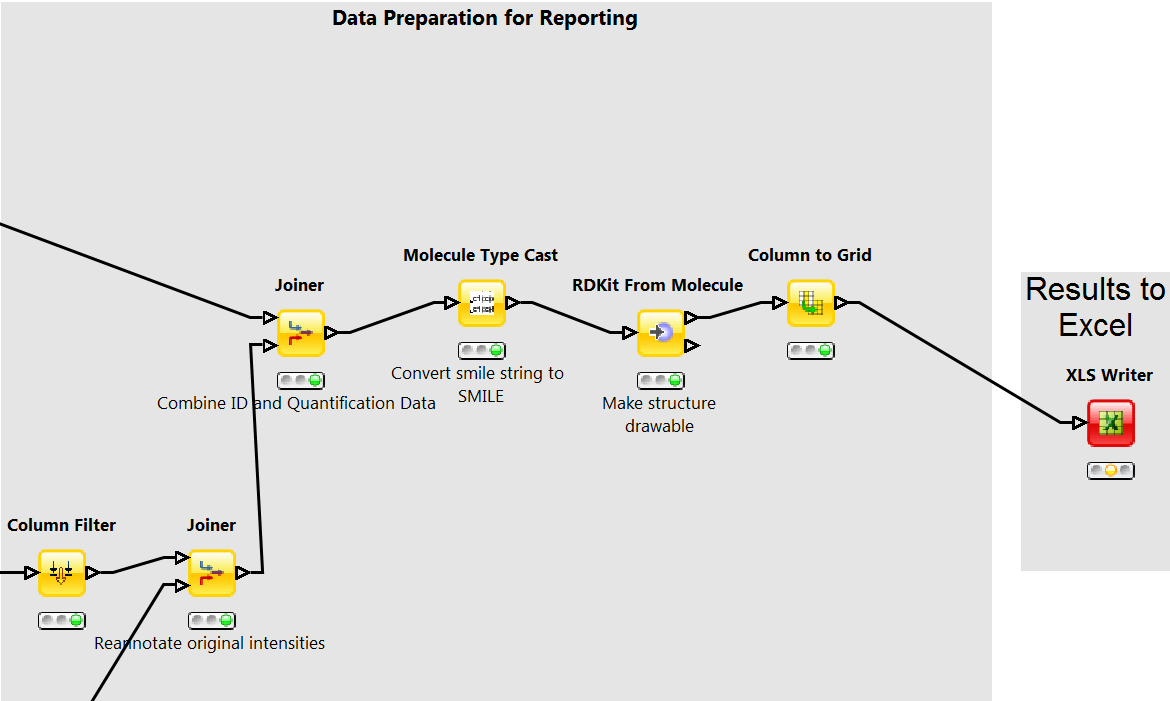
\includegraphics[width=0.7\textwidth]{graphics/metabo/reporting_2015.png}
  \caption{Data preparation for reporting}
  \label{fig:reporting}
\end{figure}

\begin{question}
What happens if we use a \textit{Left Outer Join}, \textit{Right Outer Join} or \textit{Full Outer Join} instead of the \textit{Inner Join}?
\end{question}

\begin{task}
Inspect the output of the join operation after the Molecule Type Cast and RDKit molecular structure generation.
\end{task}

While all relevant information is now contained in our table the presentation could be improved.
Currently, we have several rows corresponding to a single consensus feature (=linked feature) but with different, alternative identifications.
It would be more convenient to have only one row for each consensus feature with all accurate mass identifications added as additional columns.
To this end, we use the \KNIMENODE{Column to Grid} node that flattens several rows with the same consensus number into a single one.
Note that we have to specify the maximum number of columns in the grid so we set this to a large value (e.g. 100).
We finally export the data to an Excel file (\KNIMENODE{XLS Writer}).

